\documentclass[twoside]{book}

% Packages required by doxygen
\usepackage{fixltx2e}
\usepackage{calc}
\usepackage{doxygen}
\usepackage{graphicx}
\usepackage[utf8]{inputenc}
\usepackage{makeidx}
\usepackage{multicol}
\usepackage{multirow}
\PassOptionsToPackage{warn}{textcomp}
\usepackage{textcomp}
\usepackage[nointegrals]{wasysym}
\usepackage[table]{xcolor}
\usepackage{ifpdf,ifxetex}

% Font selection
\usepackage[T1]{fontenc}
\usepackage[scaled=.90]{helvet}
\usepackage{courier}
\usepackage{amssymb}
\usepackage{sectsty}
\renewcommand{\familydefault}{\sfdefault}
\allsectionsfont{%
  \fontseries{bc}\selectfont%
  \color{darkgray}%
}
\renewcommand{\DoxyLabelFont}{%
  \fontseries{bc}\selectfont%
  \color{darkgray}%
}
\newcommand{\+}{\discretionary{\mbox{\scriptsize$\hookleftarrow$}}{}{}}

% Page & text layout
\usepackage{geometry}
\geometry{%
  a4paper,%
  top=2.5cm,%
  bottom=2.5cm,%
  left=2.5cm,%
  right=2.5cm%
}
\tolerance=750
\hfuzz=15pt
\hbadness=750
\setlength{\emergencystretch}{15pt}
\setlength{\parindent}{0cm}
\setlength{\parskip}{3ex plus 2ex minus 2ex}
\makeatletter
\renewcommand{\paragraph}{%
  \@startsection{paragraph}{4}{0ex}{-1.0ex}{1.0ex}{%
    \normalfont\normalsize\bfseries\SS@parafont%
  }%
}
\renewcommand{\subparagraph}{%
  \@startsection{subparagraph}{5}{0ex}{-1.0ex}{1.0ex}{%
    \normalfont\normalsize\bfseries\SS@subparafont%
  }%
}
\makeatother

% Headers & footers
\usepackage{fancyhdr}
\pagestyle{fancyplain}
\fancyhead[LE]{\fancyplain{}{\bfseries\thepage}}
\fancyhead[CE]{\fancyplain{}{}}
\fancyhead[RE]{\fancyplain{}{\bfseries\leftmark}}
\fancyhead[LO]{\fancyplain{}{\bfseries\rightmark}}
\fancyhead[CO]{\fancyplain{}{}}
\fancyhead[RO]{\fancyplain{}{\bfseries\thepage}}
\fancyfoot[LE]{\fancyplain{}{}}
\fancyfoot[CE]{\fancyplain{}{}}
\fancyfoot[RE]{\fancyplain{}{\bfseries\scriptsize Generated by Doxygen }}
\fancyfoot[LO]{\fancyplain{}{\bfseries\scriptsize Generated by Doxygen }}
\fancyfoot[CO]{\fancyplain{}{}}
\fancyfoot[RO]{\fancyplain{}{}}
\renewcommand{\footrulewidth}{0.4pt}
\renewcommand{\chaptermark}[1]{%
  \markboth{#1}{}%
}
\renewcommand{\sectionmark}[1]{%
  \markright{\thesection\ #1}%
}

% Indices & bibliography
\usepackage{natbib}
\usepackage[titles]{tocloft}
\setcounter{tocdepth}{3}
\setcounter{secnumdepth}{5}
\makeindex

% Hyperlinks (required, but should be loaded last)
\ifpdf
  \usepackage[pdftex,pagebackref=true]{hyperref}
\else
  \ifxetex
    \usepackage[pagebackref=true]{hyperref}
  \else
    \usepackage[ps2pdf,pagebackref=true]{hyperref}
  \fi
\fi
\ifpdf
  \DeclareUnicodeCharacter{207B}{${}^{-}$}% Superscript minus
  \DeclareUnicodeCharacter{C2B2}{${}^{2}$}% Superscript two
  \DeclareUnicodeCharacter{C2B3}{${}^{3}$}% Superscript three
\else
  \catcode`\⁻=13% Superscript minus
  \def⁻{${}^{-}$}
  \catcode`\²=13% Superscript two
  \def²{${}^{2}$}
  \catcode`\³=13% Superscript three
  \def³{${}^{3}$}
\fi

\hypersetup{%
  colorlinks=true,%
  linkcolor=blue,%
  citecolor=blue,%
  unicode%
}

% Custom commands
\newcommand{\clearemptydoublepage}{%
  \newpage{\pagestyle{empty}\cleardoublepage}%
}

\usepackage{caption}
\captionsetup{labelsep=space,justification=centering,font={bf},singlelinecheck=off,skip=4pt,position=top}

\renewcommand{\numberline}[1]{#1~}
%===== C O N T E N T S =====

\begin{document}

% Titlepage & ToC
\hypersetup{pageanchor=false,
             bookmarksnumbered=true,
             pdfencoding=unicode
            }
\pagenumbering{alph}
\begin{titlepage}
\vspace*{7cm}
\begin{center}%
{\Large Reference Manual}\\
\vspace*{1cm}
{\large Generated by Doxygen 1.8.15}\\
\end{center}
\end{titlepage}
\clearemptydoublepage
\pagenumbering{roman}
\tableofcontents
\clearemptydoublepage
\pagenumbering{arabic}
\hypersetup{pageanchor=true}

%--- Begin generated contents ---
\chapter{S\+K\+IZ Voronoi Diagram Tool and Matlab Bindings for V\+O\+I\+SE Algorithm}
\label{index}\hypertarget{index}{}\hypertarget{index_intro_sec}{}\section{Introduction}\label{index_intro_sec}
The S\+K\+IZ\hypertarget{index_install_sec}{}\section{Installation}\label{index_install_sec}
\hypertarget{index_step1}{}\subsection{Step 1\+: Opening the box}\label{index_step1}
etc...\hypertarget{index_references_sec}{}\section{References}\label{index_references_sec}
\mbox{[}1\mbox{]} R. E. Sequeira and F. J. Preteux. Discrete voronoi diagrams and the skiz operator\+: a dynamic algorithm. I\+E\+EE Transactions on Pattern Analysis and Machine Intelligence, 19(10)\+:1165–1170, 1997 \mbox{[}doi\+: 10.\+1109/34.\+625128\mbox{]} 
\chapter{Test List}
\label{test}
\Hypertarget{test}

\begin{DoxyRefList}
\item[\label{test__test000001}%
\Hypertarget{test__test000001}%
Member \mbox{\hyperlink{testAddSeedCheckLambda_8cpp_a6f6d9e1d1c598e2fd6be48fee2857ca7}{T\+E\+S\+T\+\_\+\+C\+A\+SE}} (\char`\"{}\+Check whether the add\+Seed method correctly recalculates the lambda matrix\char`\"{})]Add\+Seed\+Check\+Lambda  
\item[\label{test__test000039}%
\Hypertarget{test__test000039}%
Member \mbox{\hyperlink{testSqDist_8cpp_a1459b5b0f8571a2db01b42527c47bc83}{T\+E\+S\+T\+\_\+\+C\+A\+SE}} (\char`\"{}\+Check squared distance between points, some of which have negative coordinates\char`\"{})]Squared\+Distance\+Negative\+Points  
\item[\label{test__test000038}%
\Hypertarget{test__test000038}%
Member \mbox{\hyperlink{testSqDist_8cpp_a4fc8b41fa1ef75ec4be9a17e144cb235}{T\+E\+S\+T\+\_\+\+C\+A\+SE}} (\char`\"{}\+Check squared distance between points which are neither vertically nor horizontally aligned\char`\"{})]Squared\+Distance\+Non\+Aligned\+Points  
\item[\label{test__test000037}%
\Hypertarget{test__test000037}%
Member \mbox{\hyperlink{testSqDist_8cpp_a84ff6dd45af7139f3cef303df1efaa41}{T\+E\+S\+T\+\_\+\+C\+A\+SE}} (\char`\"{}\+Check squared distance between points with non-\/integer coordinates\char`\"{})]Squared\+Distance\+Non\+Integer\+Points  
\item[\label{test__test000036}%
\Hypertarget{test__test000036}%
Member \mbox{\hyperlink{testSqDist_8cpp_a1ea6a49ba5e71acdd429ec3f31272298}{T\+E\+S\+T\+\_\+\+C\+A\+SE}} (\char`\"{}\+Check squared distance on horizontally aligned points\char`\"{})]Squared\+Distance\+Horizontal\+Points  
\item[\label{test__test000035}%
\Hypertarget{test__test000035}%
Member \mbox{\hyperlink{testSqDist_8cpp_ae0ea2c38f9c778654a017418d1d0b818}{T\+E\+S\+T\+\_\+\+C\+A\+SE}} (\char`\"{}\+Check squared distance on vertically aligned points\char`\"{})]Squared\+Distance\+Vertical\+Points  
\item[\label{test__test000034}%
\Hypertarget{test__test000034}%
Member \mbox{\hyperlink{testSqDist_8cpp_afab3f0de5892e92cd68fec3e1bb64e91}{T\+E\+S\+T\+\_\+\+C\+A\+SE}} (\char`\"{}\+Square distance of identical points\char`\"{})]Squared\+Distance\+Identical\+Points  
\item[\label{test__test000033}%
\Hypertarget{test__test000033}%
Member \mbox{\hyperlink{testRemoveSeedCheckV_8cpp_ac4fde08fa6ff2b060755fb556fac16aa}{T\+E\+S\+T\+\_\+\+C\+A\+SE}} (\char`\"{}\+Check whether the remove\+Seed method correctly recalculates the \char`\"{} \char`\"{}v matrix\char`\"{})]Remove\+Seed\+CheckV  
\item[\label{test__test000032}%
\Hypertarget{test__test000032}%
Member \mbox{\hyperlink{testRemoveSeedCheckLambda_8cpp_ae209f45de0f99810ba0989d65a38fc2a}{T\+E\+S\+T\+\_\+\+C\+A\+SE}} (\char`\"{}\+Check whether the remove\+Seed method correctly recalculates the lambda\char`\"{} \char`\"{} matrix\char`\"{})]Remove\+Seed\+Check\+Lambda  
\item[\label{test__test000031}%
\Hypertarget{test__test000031}%
Member \mbox{\hyperlink{testProposition2_8cpp_a4e168a9315d933cb3c6990d13a92a766}{T\+E\+S\+T\+\_\+\+C\+A\+SE}} (\char`\"{}\+Adds and then removes seeds to and from a regular grid to check \char`\"{} \char`\"{}implementation of proposition 2 in \mbox{[}1\mbox{]}\char`\"{})]Proposition2\+Check  
\item[\label{test__test000030}%
\Hypertarget{test__test000030}%
Member \mbox{\hyperlink{testPointInRegion_8cpp_a52252a02ec7fcb1f3cb79466e327e4ff}{T\+E\+S\+T\+\_\+\+C\+A\+SE}} (\char`\"{}\+Upper bounds of get\+Region\char`\"{})]Get\+Region\+Upper\+Bound  
\item[\label{test__test000029}%
\Hypertarget{test__test000029}%
Member \mbox{\hyperlink{testPointInRegion_8cpp_ab16d1b181deb76534bd83bf7d64e3b09}{T\+E\+S\+T\+\_\+\+C\+A\+SE}} (\char`\"{}\+Lower bounds of get\+Region\char`\"{})]Get\+Region\+Lower\+Bound  
\item[\label{test__test000028}%
\Hypertarget{test__test000028}%
Member \mbox{\hyperlink{testMetrics_8cpp_a5e5467d143df7d68b83a3db0e75317f2}{T\+E\+S\+T\+\_\+\+C\+A\+SE}} (\char`\"{}\+Check calculation of standard deviation of non-\/integer reals\char`\"{})]Std\+Dev\+Non\+Integer\+Vector  
\item[\label{test__test000027}%
\Hypertarget{test__test000027}%
Member \mbox{\hyperlink{testMetrics_8cpp_af5322678aa48f421f73a81ebb72478d5}{T\+E\+S\+T\+\_\+\+C\+A\+SE}} (\char`\"{}\+Check calculation of standard deviation of positive and negative numbers\char`\"{})]Std\+Dev\+Pos\+Neg\+Vector  
\item[\label{test__test000026}%
\Hypertarget{test__test000026}%
Member \mbox{\hyperlink{testMetrics_8cpp_a38c32db772d66c7927751280ff3d8aed}{T\+E\+S\+T\+\_\+\+C\+A\+SE}} (\char`\"{}\+Check calculation of standard deviation of singularly occupied vector\char`\"{})]Std\+Dev\+Single\+Vector  
\item[\label{test__test000025}%
\Hypertarget{test__test000025}%
Member \mbox{\hyperlink{testMetrics_8cpp_a11c67248a68ab4b388ad6a512290571b}{T\+E\+S\+T\+\_\+\+C\+A\+SE}} (\char`\"{}\+Check standard deviation of empty vector\char`\"{})]Std\+Dev\+Empty\+Vector  
\item[\label{test__test000024}%
\Hypertarget{test__test000024}%
Member \mbox{\hyperlink{testMetrics_8cpp_a3b9ad1a9226d6475afa62660d79a2e75}{T\+E\+S\+T\+\_\+\+C\+A\+SE}} (\char`\"{}\+Check calculation of range of non-\/integer reals\char`\"{})]Range\+Non\+Integer\+Vector  
\item[\label{test__test000023}%
\Hypertarget{test__test000023}%
Member \mbox{\hyperlink{testMetrics_8cpp_ad5e0fee1e778479d616f9db505b1604c}{T\+E\+S\+T\+\_\+\+C\+A\+SE}} (\char`\"{}\+Check calculation of range of positive and negative numbers\char`\"{})]Range\+Pos\+Neg\+Vector  
\item[\label{test__test000022}%
\Hypertarget{test__test000022}%
Member \mbox{\hyperlink{testMetrics_8cpp_a9a1728a8603b5d5d93d66958e3edac07}{T\+E\+S\+T\+\_\+\+C\+A\+SE}} (\char`\"{}\+Check calculation of range of singularly occupied vector\char`\"{})]Range\+Single\+Vector  
\item[\label{test__test000021}%
\Hypertarget{test__test000021}%
Member \mbox{\hyperlink{testMetrics_8cpp_ae4e75ab4f6bbf2508894636e864ca5fa}{T\+E\+S\+T\+\_\+\+C\+A\+SE}} (\char`\"{}\+Check range of empty vector\char`\"{})]Range\+Empty\+Vector  
\item[\label{test__test000020}%
\Hypertarget{test__test000020}%
Member \mbox{\hyperlink{testMetrics_8cpp_aa08764ae97194a58f3e0538a50508789}{T\+E\+S\+T\+\_\+\+C\+A\+SE}} (\char`\"{}\+Check sqrt\+Len of longer vector\char`\"{})]Sqrt\+Len\+Vector  
\item[\label{test__test000019}%
\Hypertarget{test__test000019}%
Member \mbox{\hyperlink{testMetrics_8cpp_a74f6b459e9d50d4dd61636b961375d23}{T\+E\+S\+T\+\_\+\+C\+A\+SE}} (\char`\"{}\+Check sqrt\+Len of singularly occupied vector\char`\"{})]Sqrt\+Len\+Single\+Vector  
\item[\label{test__test000018}%
\Hypertarget{test__test000018}%
Member \mbox{\hyperlink{testMetrics_8cpp_af8ddf1c9d577df4c55c09fe60559d54b}{T\+E\+S\+T\+\_\+\+C\+A\+SE}} (\char`\"{}\+Check sqrt\+Len of empty vector\char`\"{})]Sqrt\+Len\+Emtpy\+Vector  
\item[\label{test__test000017}%
\Hypertarget{test__test000017}%
Member \mbox{\hyperlink{testMetrics_8cpp_ab70630a1c4e94d345bb446540949dd49}{T\+E\+S\+T\+\_\+\+C\+A\+SE}} (\char`\"{}\+Check calculation of median of non-\/integer reals\char`\"{})]Median\+Non\+Integer\+Vector  
\item[\label{test__test000016}%
\Hypertarget{test__test000016}%
Member \mbox{\hyperlink{testMetrics_8cpp_a7551e1fd55f4618e1cc92780505b3a6b}{T\+E\+S\+T\+\_\+\+C\+A\+SE}} (\char`\"{}\+Check calculation of median of positive and negative numbers\char`\"{})]Median\+Pos\+Neg\+Vector  
\item[\label{test__test000015}%
\Hypertarget{test__test000015}%
Member \mbox{\hyperlink{testMetrics_8cpp_abd0df56b26da56246dade8d85f0087d5}{T\+E\+S\+T\+\_\+\+C\+A\+SE}} (\char`\"{}\+Check calculation of median of singularly occupied vector\char`\"{})]Median\+Single\+Vector  
\item[\label{test__test000014}%
\Hypertarget{test__test000014}%
Member \mbox{\hyperlink{testMetrics_8cpp_a948f7e9e3108174b8f6e15bf2d7f4f5b}{T\+E\+S\+T\+\_\+\+C\+A\+SE}} (\char`\"{}\+Check median of empty vector\char`\"{})]Median\+Empty\+Vector  
\item[\label{test__test000013}%
\Hypertarget{test__test000013}%
Member \mbox{\hyperlink{testMetrics_8cpp_ab8fba31dc7948d43cb36264f9d3aba47}{T\+E\+S\+T\+\_\+\+C\+A\+SE}} (\char`\"{}\+Check calculation of mean of non-\/integer reals\char`\"{})]Mean\+Non\+Integer\+Vector  
\item[\label{test__test000012}%
\Hypertarget{test__test000012}%
Member \mbox{\hyperlink{testMetrics_8cpp_a13bb2aad3f316b98c0f11f1ee75638a7}{T\+E\+S\+T\+\_\+\+C\+A\+SE}} (\char`\"{}\+Check calculation of mean of positive and negative numbers\char`\"{})]Mean\+Pos\+Neg\+Vector  
\item[\label{test__test000011}%
\Hypertarget{test__test000011}%
Member \mbox{\hyperlink{testMetrics_8cpp_abc0faf381e8be0f5cb380e5e98bec6fb}{T\+E\+S\+T\+\_\+\+C\+A\+SE}} (\char`\"{}\+Check calculation of mean of singularly occupied vector\char`\"{})]Mean\+Single\+Vector  
\item[\label{test__test000010}%
\Hypertarget{test__test000010}%
Member \mbox{\hyperlink{testMetrics_8cpp_a1fbdee19f95428597d27fb6435bffb77}{T\+E\+S\+T\+\_\+\+C\+A\+SE}} (\char`\"{}\+Check mean of empty vector\char`\"{})]Mean\+Emtpy\+Vector  
\item[\label{test__test000009}%
\Hypertarget{test__test000009}%
Member \mbox{\hyperlink{testInVector_8cpp_a4ebdff9874646946a45f31b1ea14e927}{T\+E\+S\+T\+\_\+\+C\+A\+SE}} (\char`\"{}\+Check if in\+Vector can handle empty vectors\char`\"{})]In\+Empty\+Vector  
\item[\label{test__test000008}%
\Hypertarget{test__test000008}%
Member \mbox{\hyperlink{testInVector_8cpp_a91b3c03c3624ce98c20e36298033c6ea}{T\+E\+S\+T\+\_\+\+C\+A\+SE}} (\char`\"{}\+Check if in\+Vector correctly identifies lack of item in vector of\char`\"{} \char`\"{}reals\char`\"{})]Not\+In\+Vector\+Of\+Reals  
\item[\label{test__test000007}%
\Hypertarget{test__test000007}%
Member \mbox{\hyperlink{testInVector_8cpp_a61ce30f01fbb56b1c24eea5b9f565bdb}{T\+E\+S\+T\+\_\+\+C\+A\+SE}} (\char`\"{}\+Check if in\+Vector correctly identifies item in vector of reals\char`\"{})]In\+Vector\+Of\+Reals  
\item[\label{test__test000006}%
\Hypertarget{test__test000006}%
Member \mbox{\hyperlink{testInVector_8cpp_ac0090be73626bcf546b5398e8328ae6c}{T\+E\+S\+T\+\_\+\+C\+A\+SE}} (\char`\"{}\+Check if in\+Vector correctly identifies lack of item in vector of\char`\"{} \char`\"{}ints\char`\"{})]Not\+In\+Vector\+Of\+Ints  
\item[\label{test__test000005}%
\Hypertarget{test__test000005}%
Member \mbox{\hyperlink{testInVector_8cpp_ab34965ac493a2cdf51939266c8ffa019}{T\+E\+S\+T\+\_\+\+C\+A\+SE}} (\char`\"{}\+Check if in\+Vector correctly identifies item in vector of ints\char`\"{})]In\+Vector\+Of\+Ints  
\item[\label{test__test000004}%
\Hypertarget{test__test000004}%
Member \mbox{\hyperlink{testGetVDOp_8cpp_ac94dd5a8833ccee72d795c3075dca240}{T\+E\+S\+T\+\_\+\+C\+A\+SE}} (\char`\"{}\+Checks that the get\+V\+D\+Op function correctly returns a matrix of\char`\"{} \char`\"{}averages from V\+D and pixel intensity data\char`\"{})]Get\+V\+D\+Op\+Median  
\item[\label{test__test000003}%
\Hypertarget{test__test000003}%
Member \mbox{\hyperlink{testGetCentroid_8cpp_aaf22362ddc2184c36c8e84dabc3f43e7}{T\+E\+S\+T\+\_\+\+C\+A\+SE}} (\char`\"{}\+Checks that the get\+V\+D\+Op function correctly returns a matrix of \char`\"{} \char`\"{}averages from V\+D and pixel intensity data\char`\"{})]Get\+Centroid\+Check  
\item[\label{test__test000002}%
\Hypertarget{test__test000002}%
Member \mbox{\hyperlink{testAddSeedCheckV_8cpp_a1475bb67182d67e8d4aaaa1a9d887e65}{T\+E\+S\+T\+\_\+\+C\+A\+SE}} (\char`\"{}\+Check whether the add\+Seed method correctly recalculates the v\char`\"{} \char`\"{}matrix.\char`\"{})]Add\+Seed\+CheckV 
\end{DoxyRefList}
\chapter{Module Index}
\section{Global Functions}
All non class method functions (links contain more details)\+:\begin{DoxyCompactList}
\item \contentsline{section}{add\+Seed}{\pageref{group__addSeed}}{}
\item \contentsline{section}{get\+Region}{\pageref{group__getRegion}}{}
\item \contentsline{section}{grab\+VD}{\pageref{group__grabVD}}{}
\item \contentsline{section}{ns\+Star}{\pageref{group__nsStar}}{}
\item \contentsline{section}{point\+In\+Region}{\pageref{group__pointInRegion}}{}
\item \contentsline{section}{push\+VD}{\pageref{group__pushVD}}{}
\item \contentsline{section}{circumcentre}{\pageref{group__circumcentre}}{}
\item \contentsline{section}{in\+Vector}{\pageref{group__inVector}}{}
\item \contentsline{section}{read\+Matrix}{\pageref{group__readMatrix}}{}
\item \contentsline{section}{read\+Seeds}{\pageref{group__readSeeds}}{}
\item \contentsline{section}{sq\+Dist}{\pageref{group__sqDist}}{}
\item \contentsline{section}{update\+Dict}{\pageref{group__updateDict}}{}
\end{DoxyCompactList}

\chapter{Hierarchical Index}
\section{Class Hierarchy}
This inheritance list is sorted roughly, but not completely, alphabetically\+:\begin{DoxyCompactList}
\item exception\begin{DoxyCompactList}
\item \contentsline{section}{S\+K\+I\+Z\+Exception}{\pageref{classSKIZException}}{}
\begin{DoxyCompactList}
\item \contentsline{section}{S\+K\+I\+Z\+Identical\+Seeds\+Exception}{\pageref{classSKIZIdenticalSeedsException}}{}
\item \contentsline{section}{S\+K\+I\+Z\+Index\+Exception}{\pageref{classSKIZIndexException}}{}
\item \contentsline{section}{S\+K\+I\+Z\+I\+O\+Exception}{\pageref{classSKIZIOException}}{}
\item \contentsline{section}{S\+K\+I\+Z\+Linear\+Seeds\+Exception}{\pageref{classSKIZLinearSeedsException}}{}
\end{DoxyCompactList}
\end{DoxyCompactList}
\item \contentsline{section}{V\+\_\+struct}{\pageref{structV__struct}}{}
\item \contentsline{section}{vd}{\pageref{classvd}}{}
\item \contentsline{section}{W\+\_\+struct}{\pageref{structW__struct}}{}
\end{DoxyCompactList}

\chapter{Data Structure Index}
\section{Data Structures}
Here are the data structures with brief descriptions\+:\begin{DoxyCompactList}
\item\contentsline{section}{\mbox{\hyperlink{classSKIZException}{S\+K\+I\+Z\+Exception}} \\*Parent class for all S\+K\+IZ exceptions }{\pageref{classSKIZException}}{}
\item\contentsline{section}{\mbox{\hyperlink{classSKIZIdenticalSeedsException}{S\+K\+I\+Z\+Identical\+Seeds\+Exception}} \\*Thrown if add\+Seed is given a seed to add to Voronoi diagram where one already exists }{\pageref{classSKIZIdenticalSeedsException}}{}
\item\contentsline{section}{\mbox{\hyperlink{classSKIZIndexException}{S\+K\+I\+Z\+Index\+Exception}} \\*Thrown when trying to access a non-\/existent entry in a std\+::vector or std\+::map }{\pageref{classSKIZIndexException}}{}
\item\contentsline{section}{\mbox{\hyperlink{classSKIZIOException}{S\+K\+I\+Z\+I\+O\+Exception}} \\*Thrown in case of failure to open a file for reading or writing }{\pageref{classSKIZIOException}}{}
\item\contentsline{section}{\mbox{\hyperlink{classSKIZLinearSeedsException}{S\+K\+I\+Z\+Linear\+Seeds\+Exception}} \\*Thrown by circumcentre if input coordinates form a line }{\pageref{classSKIZLinearSeedsException}}{}
\item\contentsline{section}{\mbox{\hyperlink{structV__struct}{V\+\_\+struct}} \\*As defined in \mbox{[}1\mbox{]}, Section 3 (Vk) }{\pageref{structV__struct}}{}
\item\contentsline{section}{\mbox{\hyperlink{classvd}{vd}} \\*Contains all information about voronoi diagram needed to perform S\+K\+IZ algorithm from \mbox{[}1\mbox{]} }{\pageref{classvd}}{}
\item\contentsline{section}{\mbox{\hyperlink{structW__struct}{W\+\_\+struct}} \\*As defined in \mbox{[}1\mbox{]}, Section 2.\+2. Only for use with V\+O\+I\+SE algorithm Matlab interface. Unused but here for consistency }{\pageref{structW__struct}}{}
\end{DoxyCompactList}

\chapter{File Index}
\section{File List}
Here is a list of all documented files with brief descriptions\+:\begin{DoxyCompactList}
\item\contentsline{section}{src/\mbox{\hyperlink{addSeed_8cpp}{add\+Seed.\+cpp}} \\*Adds seed to Voronoi diagram }{\pageref{addSeed_8cpp}}{}
\item\contentsline{section}{src/\mbox{\hyperlink{addSeed_8h}{add\+Seed.\+h}} }{\pageref{addSeed_8h}}{}
\item\contentsline{section}{src/\mbox{\hyperlink{getCentroid_8cpp}{get\+Centroid.\+cpp}} \\*Find the centres of mass for multiple V\+Rs in a VD }{\pageref{getCentroid_8cpp}}{}
\item\contentsline{section}{src/{\bfseries get\+Centroid.\+h} }{\pageref{getCentroid_8h}}{}
\item\contentsline{section}{src/\mbox{\hyperlink{getOp_8cpp}{get\+Op.\+cpp}} \\*Finds average pixel intensity of all V\+Rs in VD }{\pageref{getOp_8cpp}}{}
\item\contentsline{section}{src/{\bfseries get\+Op.\+h} }{\pageref{getOp_8h}}{}
\item\contentsline{section}{src/\mbox{\hyperlink{getRegion_8cpp}{get\+Region.\+cpp}} \\*Finds the Voronoi region R(s) of a seed s }{\pageref{getRegion_8cpp}}{}
\item\contentsline{section}{src/\mbox{\hyperlink{getRegion_8h}{get\+Region.\+h}} }{\pageref{getRegion_8h}}{}
\item\contentsline{section}{src/\mbox{\hyperlink{NSStar_8cpp}{N\+S\+Star.\+cpp}} \\*Finds neighbouring Voronoi regions for new seeds }{\pageref{NSStar_8cpp}}{}
\item\contentsline{section}{src/\mbox{\hyperlink{NSStar_8h}{N\+S\+Star.\+h}} }{\pageref{NSStar_8h}}{}
\item\contentsline{section}{src/\mbox{\hyperlink{pointInRegion_8cpp}{point\+In\+Region.\+cpp}} \\*Checks whether a point is within region C(s, A) according to \mbox{[}1\mbox{]} definition 2.\+5 }{\pageref{pointInRegion_8cpp}}{}
\item\contentsline{section}{src/\mbox{\hyperlink{pointInRegion_8h}{point\+In\+Region.\+h}} \\*Checks whether a point is within region C(s, A) according to \mbox{[}1\mbox{]} definition 2.\+5. }{\pageref{pointInRegion_8h}}{}
\item\contentsline{section}{src/\mbox{\hyperlink{removeSeed_8cpp}{remove\+Seed.\+cpp}} \\*Removes seed from Voronoi diagram }{\pageref{removeSeed_8cpp}}{}
\item\contentsline{section}{src/\mbox{\hyperlink{removeSeed_8h}{remove\+Seed.\+h}} }{\pageref{removeSeed_8h}}{}
\item\contentsline{section}{src/\mbox{\hyperlink{skizException_8cpp}{skiz\+Exception.\+cpp}} \\*Exception class for S\+K\+IZ Operator Tool }{\pageref{skizException_8cpp}}{}
\item\contentsline{section}{src/\mbox{\hyperlink{skizException_8h}{skiz\+Exception.\+h}} }{\pageref{skizException_8h}}{}
\item\contentsline{section}{src/\mbox{\hyperlink{typedefs_8h}{typedefs.\+h}} \\*Type definitions (all in one place) }{\pageref{typedefs_8h}}{}
\item\contentsline{section}{src/\mbox{\hyperlink{vd_8cpp}{vd.\+cpp}} \\*Voronoi diagram class }{\pageref{vd_8cpp}}{}
\item\contentsline{section}{src/\mbox{\hyperlink{vd_8h}{vd.\+h}} }{\pageref{vd_8h}}{}
\item\contentsline{section}{src/aux-\/functions/\mbox{\hyperlink{arrayPosInVector_8h}{array\+Pos\+In\+Vector.\+h}} \\*Function to check whether coordinate array exists in vector of coordinate arrays }{\pageref{arrayPosInVector_8h}}{}
\item\contentsline{section}{src/aux-\/functions/\mbox{\hyperlink{circumcentre_8h}{circumcentre.\+h}} \\*Finds the cirumcentre of the triangle formed by three given points (templated). Header only for templating/linking reasons }{\pageref{circumcentre_8h}}{}
\item\contentsline{section}{src/aux-\/functions/\mbox{\hyperlink{inVector_8h}{in\+Vector.\+h}} \\*Checks whether item exists within a vector. Header only for templating/linking reasons }{\pageref{inVector_8h}}{}
\item\contentsline{section}{src/aux-\/functions/\mbox{\hyperlink{metrics_8cpp}{metrics.\+cpp}} \\*Series of metrics to be used in get\+V\+D\+Op (substitute for Matlab\textquotesingle{}s ability to pass function handles as arguments). Used in V\+O\+I\+SE }{\pageref{metrics_8cpp}}{}
\item\contentsline{section}{src/aux-\/functions/\mbox{\hyperlink{metrics_8h}{metrics.\+h}} }{\pageref{metrics_8h}}{}
\item\contentsline{section}{src/aux-\/functions/\mbox{\hyperlink{proposition2_8cpp}{proposition2.\+cpp}} \\*Uses proposition 2 to decide between seeds for addition to N(s$\ast$) }{\pageref{proposition2_8cpp}}{}
\item\contentsline{section}{src/aux-\/functions/{\bfseries proposition2.\+h} }{\pageref{proposition2_8h}}{}
\item\contentsline{section}{src/aux-\/functions/\mbox{\hyperlink{readMatrix_8cpp}{read\+Matrix.\+cpp}} \\*Reads matrix from ascii-\/formatted files generated by Matlab\textquotesingle{}s \textquotesingle{}save\textquotesingle{} function }{\pageref{readMatrix_8cpp}}{}
\item\contentsline{section}{src/aux-\/functions/\mbox{\hyperlink{readMatrix_8h}{read\+Matrix.\+h}} }{\pageref{readMatrix_8h}}{}
\item\contentsline{section}{src/aux-\/functions/\mbox{\hyperlink{readSeeds_8cpp}{read\+Seeds.\+cpp}} \\*Reads seed coordinates from ascii-\/formatted files generated by Matlab\textquotesingle{}s \textquotesingle{}save\textquotesingle{} function }{\pageref{readSeeds_8cpp}}{}
\item\contentsline{section}{src/aux-\/functions/\mbox{\hyperlink{readSeeds_8h}{read\+Seeds.\+h}} }{\pageref{readSeeds_8h}}{}
\item\contentsline{section}{src/aux-\/functions/\mbox{\hyperlink{sqDist_8h}{sq\+Dist.\+h}} \\*Finds the squared difference between two points (templated). Header only for templating/linking reasons }{\pageref{sqDist_8h}}{}
\item\contentsline{section}{src/aux-\/functions/\mbox{\hyperlink{updateDict_8h}{update\+Dict.\+h}} \\*Routine for adding to the vector in a dictionary of vectors only if the item does not already exist (templated). Header only for templating/linking reasons }{\pageref{updateDict_8h}}{}
\item\contentsline{section}{src/mex/\mbox{\hyperlink{addSeedToVD_8cpp}{add\+Seed\+To\+V\+D.\+cpp}} \\*This is a M\+EX function. It should only be compiled by the compile\+M\+E\+X.\+m matlab script. Adds single seeds to Voronoi diagram }{\pageref{addSeedToVD_8cpp}}{}
\item\contentsline{section}{src/mex/\mbox{\hyperlink{addSeedToVDBatch_8cpp}{add\+Seed\+To\+V\+D\+Batch.\+cpp}} \\*This is a M\+EX function. It should only be compiled by the compile\+M\+E\+X.\+m matlab script. Adds multiple seeds to Voronoi diagram }{\pageref{addSeedToVDBatch_8cpp}}{}
\item\contentsline{section}{src/mex/\mbox{\hyperlink{getCentroidSeedBatch_8cpp}{get\+Centroid\+Seed\+Batch.\+cpp}} \\*This is a M\+EX function. It should only be compiled by the compile\+M\+E\+X.\+m matlab script. Finds the pixel-\/intensity weighted centre of mass for all V\+Rs in a VD }{\pageref{getCentroidSeedBatch_8cpp}}{}
\item\contentsline{section}{src/mex/\mbox{\hyperlink{getVDOp_8cpp}{get\+V\+D\+Op.\+cpp}} \\*This is a M\+EX function. It should only be compiled by the compile\+M\+E\+X.\+m Matlab script. Uses one of six metrics (mean, median, standard deviation, range, normalised range, number of pixels) to evaluate the merit function of a Voronoi region }{\pageref{getVDOp_8cpp}}{}
\item\contentsline{section}{src/mex/\mbox{\hyperlink{grabVD_8cpp}{grab\+V\+D.\+cpp}} \\*This is a M\+EX function. It should only be compiled by the compile\+M\+E\+X.\+m Matlab script. Allocates memory and populates vd object with data from Matlab VD struct. Only for use with Matlab mex compiler }{\pageref{grabVD_8cpp}}{}
\item\contentsline{section}{src/mex/\mbox{\hyperlink{grabVD_8h}{grab\+V\+D.\+h}} }{\pageref{grabVD_8h}}{}
\item\contentsline{section}{src/mex/\mbox{\hyperlink{grabW_8cpp}{grab\+W.\+cpp}} \\*This is a requirement for a M\+EX function. It should only be compiled by the compile\+M\+E\+X.\+m Matlab script. Gets params.\+W matrix from VD Matlab struct }{\pageref{grabW_8cpp}}{}
\item\contentsline{section}{src/mex/\mbox{\hyperlink{grabW_8h}{grab\+W.\+h}} }{\pageref{grabW_8h}}{}
\item\contentsline{section}{src/mex/\mbox{\hyperlink{mexIncludes_8h}{mex\+Includes.\+h}} \\*All includes for M\+EX functions. All files here have include guards }{\pageref{mexIncludes_8h}}{}
\item\contentsline{section}{src/mex/\mbox{\hyperlink{pushVD_8cpp}{push\+V\+D.\+cpp}} \\*This is a requirement for a M\+EX function. It should only be compiled by the compile\+M\+E\+X.\+m Matlab script. Allocates memory and populates Matlab struct with data from vd object. Only for use with Matlab mex compiler }{\pageref{pushVD_8cpp}}{}
\item\contentsline{section}{src/mex/\mbox{\hyperlink{pushVD_8h}{push\+V\+D.\+h}} }{\pageref{pushVD_8h}}{}
\item\contentsline{section}{src/mex/\mbox{\hyperlink{removeSeedFromVD_8cpp}{remove\+Seed\+From\+V\+D.\+cpp}} \\*This is a M\+EX function. It should only be compiled by the compile\+M\+E\+X.\+m matlab script. Removes single seed from Voronoi diagram }{\pageref{removeSeedFromVD_8cpp}}{}
\item\contentsline{section}{src/mex/\mbox{\hyperlink{removeSeedFromVDBatch_8cpp}{remove\+Seed\+From\+V\+D\+Batch.\+cpp}} \\*This is a M\+EX function. It should only be compiled by the compile\+M\+E\+X.\+m matlab script. Removes multiple seeds from Voronoi diagram }{\pageref{removeSeedFromVDBatch_8cpp}}{}
\item\contentsline{section}{src/mex/\mbox{\hyperlink{sopToWop_8cpp}{sop\+To\+Wop.\+cpp}} \\*Takes a vector of values with which to populate each VR with for displaying clustering results }{\pageref{sopToWop_8cpp}}{}
\item\contentsline{section}{src/test/\mbox{\hyperlink{testAddSeedCheckLambda_8cpp}{test\+Add\+Seed\+Check\+Lambda.\+cpp}} \\*Unit tests for whether the add\+Seed method correctly recalculates the $ \lambda $ matrix }{\pageref{testAddSeedCheckLambda_8cpp}}{}
\item\contentsline{section}{src/test/\mbox{\hyperlink{testAddSeedCheckV_8cpp}{test\+Add\+Seed\+Check\+V.\+cpp}} \\*Unit tests for whether the add\+Seed method correctly recalculates the $ \nu $ matrix }{\pageref{testAddSeedCheckV_8cpp}}{}
\item\contentsline{section}{src/test/\mbox{\hyperlink{testGetCentroid_8cpp}{test\+Get\+Centroid.\+cpp}} \\*Unit tests for whether the get\+Centroid function correctly returns the centres of mass of the V\+Rs }{\pageref{testGetCentroid_8cpp}}{}
\item\contentsline{section}{src/test/\mbox{\hyperlink{testGetVDOp_8cpp}{test\+Get\+V\+D\+Op.\+cpp}} \\*Unit tests for whether the get\+V\+D\+Op function correctly calculates the average intensity for each VR }{\pageref{testGetVDOp_8cpp}}{}
\item\contentsline{section}{src/test/\mbox{\hyperlink{testInVector_8cpp}{test\+In\+Vector.\+cpp}} \\*Unit tests for whether in\+Vector correctly identifies the presence or otherwise of numeric values in vectors }{\pageref{testInVector_8cpp}}{}
\item\contentsline{section}{src/test/\mbox{\hyperlink{testMetrics_8cpp}{test\+Metrics.\+cpp}} \\*Unit tests for the metrics used in \mbox{\hyperlink{getVDOp_8cpp}{get\+V\+D\+Op.\+cpp}} M\+EX function }{\pageref{testMetrics_8cpp}}{}
\item\contentsline{section}{src/test/\mbox{\hyperlink{testPointInRegion_8cpp}{test\+Point\+In\+Region.\+cpp}} \\*Unit tests for various normal and pathalogical cases for the point\+In\+Region function }{\pageref{testPointInRegion_8cpp}}{}
\item\contentsline{section}{src/test/\mbox{\hyperlink{testProposition2_8cpp}{test\+Proposition2.\+cpp}} \\*Unit test\+: Adds and then removes seeds to and from a regular grid to check implementation of proposition 2 in \mbox{[}1\mbox{]} }{\pageref{testProposition2_8cpp}}{}
\item\contentsline{section}{src/test/\mbox{\hyperlink{testRemoveSeedCheckLambda_8cpp}{test\+Remove\+Seed\+Check\+Lambda.\+cpp}} \\*Unit tests for whether the remove\+Seed method correctly recalculates the $ \lambda $ matrix }{\pageref{testRemoveSeedCheckLambda_8cpp}}{}
\item\contentsline{section}{src/test/\mbox{\hyperlink{testRemoveSeedCheckV_8cpp}{test\+Remove\+Seed\+Check\+V.\+cpp}} \\*Unit tests for whether the remove\+Seed method correctly recalculates the $ \nu $ matrix }{\pageref{testRemoveSeedCheckV_8cpp}}{}
\item\contentsline{section}{src/test/\mbox{\hyperlink{testSqDist_8cpp}{test\+Sq\+Dist.\+cpp}} \\*Unit tests for sq\+Dist function }{\pageref{testSqDist_8cpp}}{}
\end{DoxyCompactList}

\chapter{Module Documentation}
\hypertarget{group__addSeed}{}\section{add\+Seed}
\label{group__addSeed}\index{add\+Seed@{add\+Seed}}


Adds seed to voronoi diagram.  


Adds seed to voronoi diagram. 


\begin{DoxyParams}{Parameters}
{\em VD} & vd object (definition in \mbox{\hyperlink{vd_8h}{vd.\+h}}) \\
\hline
{\em s1} & First coordinate of seed to be added \\
\hline
{\em s2} & Second coordinate of seed to be added\\
\hline
\end{DoxyParams}
Method used is taken from \char`\"{}\+Discrete Voronoi Diagrams and the S\+K\+I\+Z
 Operator\+: A Dynamic Algorithm\char`\"{} \mbox{[}1\mbox{]}, Section 3.\+1 
\hypertarget{group__getRegion}{}\section{get\+Region}
\label{group__getRegion}\index{get\+Region@{get\+Region}}


Finds the voronoi region R(s) of a seed s.  


Finds the voronoi region R(s) of a seed s. 


\begin{DoxyParams}{Parameters}
{\em VD} & Voronoi diagram \\
\hline
{\em s} & ID of seed for which R(s) is to be found \\
\hline
\end{DoxyParams}
\begin{DoxyReturn}{Returns}
(m x 2) Eigen\+::\+Array. Each row is either (-\/1, -\/1) if there are no pixels in the corresponding row in W that are also in R(s), or (lb, ub) where 0 $<$= lb $<$= ub $<$ n, indicating that the pixels in the $i^{th}$ row in the interval (lb, ub\mbox{]} are in R(s).
\end{DoxyReturn}
R(s) is as defined in \mbox{[}1\mbox{]}, Definition 1.\+1. 
\hypertarget{group__nsStar}{}\section{ns\+Star}
\label{group__nsStar}\index{ns\+Star@{ns\+Star}}


Finds neighbouring Voronoi regions for new seeds.  


Finds neighbouring Voronoi regions for new seeds. 


\begin{DoxyParams}{Parameters}
{\em VD} & Voronoi diagram \\
\hline
\end{DoxyParams}
\begin{DoxyReturn}{Returns}
Vector of the I\+Ds of seeds with Voronoi regions bordering the Voronoi region of the seed last added to the Voronoi diagram
\end{DoxyReturn}
Method used is taken from \char`\"{}\+Discrete Voronoi Diagrams and the S\+K\+I\+Z
 Operator\+: A Dynamic Algorithm\char`\"{} \mbox{[}1\mbox{]}, Section 3.\+1 
\hypertarget{group__pointInRegion}{}\section{point\+In\+Region}
\label{group__pointInRegion}\index{point\+In\+Region@{point\+In\+Region}}


Checks whether a point is within region C(s, A) according to \mbox{[}1\mbox{]} definition 2.\+5.  


Checks whether a point is within region C(s, A) according to \mbox{[}1\mbox{]} definition 2.\+5. 


\begin{DoxyParams}{Parameters}
{\em vd} & Voronoi Diagram \\
\hline
{\em pt} & x and y coordinates of point to check \\
\hline
{\em s} & Index of seed which defines the region being checked \\
\hline
{\em A} & Vector of seeds which together form half-\/planes that make up C(s, A) \\
\hline
\end{DoxyParams}
\begin{DoxyReturn}{Returns}
true\+: Point is in C(s, A) 

false\+: Point is not in C(s, A) 
\end{DoxyReturn}

\hypertarget{group__circumcentre}{}\section{circumcentre}
\label{group__circumcentre}\index{circumcentre@{circumcentre}}


Finds the cirumcentre of the triangle formed by three given points.  


Finds the cirumcentre of the triangle formed by three given points. 


\begin{DoxyParams}{Parameters}
{\em ax,ay} & x and y coordinates of first vertex \\
\hline
{\em bx,by} & x and y coordinates of second vertex \\
\hline
{\em cx,cy} & x and y coordinates of third vertex \\
\hline
\end{DoxyParams}
\begin{DoxyReturn}{Returns}
Circumcentre of points a, b and c
\end{DoxyReturn}
The cirumcentre of a triangle is the unique point in $R^2$ that is equidistant from its three vertices. This is the equivalent of X(a, b, c) as defined in Section 2 of reference \mbox{[}1\mbox{]}. 
\hypertarget{group__inVector}{}\section{in\+Vector}
\label{group__inVector}\index{in\+Vector@{in\+Vector}}


Checks whether or not item is in vector.  


\subsection*{Functions}
\begin{DoxyCompactItemize}
\item 
\mbox{\Hypertarget{group__inVector_gaff003321eb7b590593a84de0147aa6bd}\label{group__inVector_gaff003321eb7b590593a84de0147aa6bd}} 
bool {\bfseries in\+Vector} (const \mbox{\hyperlink{typedefs_8cpp_a84b6d9a0fbb45e01ad4a3aa5667f2992}{Real\+Vec}} \&vec, const \mbox{\hyperlink{typedefs_8cpp_a58a0c7cf2501f4492da833421be92547}{real}} \&item)
\end{DoxyCompactItemize}


\subsection{Detailed Description}
Checks whether or not item is in vector. 


\begin{DoxyParams}{Parameters}
{\em vec} & Vector to be checked for item \\
\hline
{\em item} & Item to be looked for \\
\hline
\end{DoxyParams}
\begin{DoxyReturn}{Returns}
true\+: item is in vector 

false\+: item is not in vector 
\end{DoxyReturn}

\hypertarget{group__readMatrix}{}\section{read\+Matrix}
\label{group__readMatrix}\index{read\+Matrix@{read\+Matrix}}


Reads matrix from ascii-\/formatted files generated by Matlab\textquotesingle{}s \textquotesingle{}save\textquotesingle{} function.  


Reads matrix from ascii-\/formatted files generated by Matlab\textquotesingle{}s \textquotesingle{}save\textquotesingle{} function. 

Use with files created by 
\begin{DoxyCode}{0}
\DoxyCodeLine{save(varName, fileName, \textcolor{stringliteral}{"-ascii"})}
\end{DoxyCode}
 in Matlab


\begin{DoxyParams}{Parameters}
{\em filename} & Name of text file to be read \\
\hline
\end{DoxyParams}
\begin{DoxyReturn}{Returns}
Eigen array with matrix from text file 
\end{DoxyReturn}

\hypertarget{group__readSeeds}{}\section{read\+Seeds}
\label{group__readSeeds}\index{read\+Seeds@{read\+Seeds}}


Reads seed coordinates from ascii-\/formatted files generated by Matlab\textquotesingle{}s \textquotesingle{}save\textquotesingle{} function.  


Reads seed coordinates from ascii-\/formatted files generated by Matlab\textquotesingle{}s \textquotesingle{}save\textquotesingle{} function. 


\begin{DoxyParams}{Parameters}
{\em filename} & Name of text file to be read \\
\hline
\end{DoxyParams}
\begin{DoxyReturn}{Returns}
Vector containing two std\+::vector$<$double$>$\+: the x and y coordinates of the seeds 
\end{DoxyReturn}

\hypertarget{group__sqDist}{}\section{sq\+Dist}
\label{group__sqDist}\index{sq\+Dist@{sq\+Dist}}


Finds the squared difference between two points.  


\subsection*{Functions}
\begin{DoxyCompactItemize}
\item 
\mbox{\Hypertarget{group__sqDist_ga18d0a77f62f604bf2ba74500658add69}\label{group__sqDist_ga18d0a77f62f604bf2ba74500658add69}} 
\mbox{\hyperlink{typedefs_8cpp_a58a0c7cf2501f4492da833421be92547}{real}} {\bfseries sq\+Dist} (const \mbox{\hyperlink{typedefs_8cpp_a58a0c7cf2501f4492da833421be92547}{real}} \&p1, const \mbox{\hyperlink{typedefs_8cpp_a58a0c7cf2501f4492da833421be92547}{real}} \&p2, const \mbox{\hyperlink{typedefs_8cpp_a58a0c7cf2501f4492da833421be92547}{real}} \&q1, const \mbox{\hyperlink{typedefs_8cpp_a58a0c7cf2501f4492da833421be92547}{real}} \&q2)
\end{DoxyCompactItemize}


\subsection{Detailed Description}
Finds the squared difference between two points. 


\begin{DoxyParams}{Parameters}
{\em p1,p2} & x and y coordinates of first point \\
\hline
{\em q1,q2} & x and y coordinates of second point \\
\hline
\end{DoxyParams}
\begin{DoxyReturn}{Returns}
Squared distance between points p and q
\end{DoxyReturn}
Using squared distance gives integer results when inputs are limited to W as defined in doi\+: 10.\+1109/34.\+625128, Section 2.\+2 which avoids floating point precision errors. 
\hypertarget{group__updateDict}{}\section{update\+Dict}
\label{group__updateDict}\index{update\+Dict@{update\+Dict}}


Custom routine for adding to the vector in a dictionary of vectors only if the item does not already exist.  


\subsection*{Functions}
\begin{DoxyCompactItemize}
\item 
void \mbox{\hyperlink{group__updateDict_gaecb9b6904667c0bde630eadf45d36835}{update\+Dict}} (std\+::map$<$ real, \mbox{\hyperlink{aux_8h_ac0a1a538b45426e056715d1f59f854ab}{Real\+Vec}} $>$ \&d, const real \&key, const real \&value)
\end{DoxyCompactItemize}


\subsection{Detailed Description}
Custom routine for adding to the vector in a dictionary of vectors only if the item does not already exist. 


\begin{DoxyParams}{Parameters}
{\em d} & Dictionary \\
\hline
{\em key} & Key to be added \\
\hline
{\em value} & Value to be added to vector \\
\hline
\end{DoxyParams}


\subsection{Function Documentation}
\mbox{\Hypertarget{group__updateDict_gaecb9b6904667c0bde630eadf45d36835}\label{group__updateDict_gaecb9b6904667c0bde630eadf45d36835}} 
\index{update\+Dict@{update\+Dict}!update\+Dict@{update\+Dict}}
\index{update\+Dict@{update\+Dict}!update\+Dict@{update\+Dict}}
\subsubsection{\texorpdfstring{update\+Dict()}{updateDict()}}
{\footnotesize\ttfamily void update\+Dict (\begin{DoxyParamCaption}\item[{std\+::map$<$ real, \mbox{\hyperlink{aux_8h_ac0a1a538b45426e056715d1f59f854ab}{Real\+Vec}} $>$ \&}]{d,  }\item[{const real \&}]{key,  }\item[{const real \&}]{value }\end{DoxyParamCaption})}

If key and corresponding vector do not exist, we create both and populate vector with value 
\hypertarget{group__mexFunctions}{}\section{Mex\+Functions}
\label{group__mexFunctions}\index{Mex\+Functions@{Mex\+Functions}}
mex\+Functions \begin{DoxyReturn}{Returns}
void 
\end{DoxyReturn}

\hypertarget{group__grabVD}{}\section{grab\+VD}
\label{group__grabVD}\index{grab\+VD@{grab\+VD}}


Allocates memory and populates vd object with data from matlab VD struct. Only for use with Matlab mex compiler.  


Allocates memory and populates vd object with data from matlab VD struct. Only for use with Matlab mex compiler. 


\begin{DoxyParams}[1]{Parameters}
\mbox{\tt in}  & {\em prhs} & Voronoi diagram in the form of a Matlab struct with the relevant fields filled in the correct manner. \\
\hline
\end{DoxyParams}
\begin{DoxyReturn}{Returns}
Voronoi diagram (vd) object containing all relevant information.
\end{DoxyReturn}
The larger matrices ( $ \lambda, \nu $ in \mbox{[}1\mbox{]} as well as px and py) are not copied but mapped using Eigen\textquotesingle{}s map class for reasons of speed.

This is part of the Matlab bindings for the V\+O\+I\+SE algorithm \mbox{[}2\mbox{]}, and is only compatible with the code written to this end by P. Guio and N. Achilleos. 
\hypertarget{group__pushVD}{}\section{push\+VD}
\label{group__pushVD}\index{push\+VD@{push\+VD}}


Allocates memory and populates Matlab struct with data from vd object. Only for use with Matlab mex compiler.  


Allocates memory and populates Matlab struct with data from vd object. Only for use with Matlab mex compiler. 


\begin{DoxyParams}[1]{Parameters}
\mbox{\tt in}  & {\em output\+VD} & Voronoi diagram from which data is read \\
\hline
\mbox{\tt out}  & {\em plhs} & Pointer to mx\+Array object which is the start of the section of memory to be populated with data and which Matlab will interpret as a struct containing all of the information from output\+VD. This is part of the Matlab bindings for the V\+O\+I\+SE algorithm \mbox{[}2\mbox{]}, and is only compatible with the code written to this end by P. Guio and N. Achilleos. \\
\hline
\end{DoxyParams}

\chapter{Data Structure Documentation}
\hypertarget{classSKIZException}{}\section{S\+K\+I\+Z\+Exception Class Reference}
\label{classSKIZException}\index{S\+K\+I\+Z\+Exception@{S\+K\+I\+Z\+Exception}}


Parent class for all S\+K\+IZ exceptions.  




{\ttfamily \#include $<$skiz\+Exception.\+h$>$}

Inheritance diagram for S\+K\+I\+Z\+Exception\+:\begin{figure}[H]
\begin{center}
\leavevmode
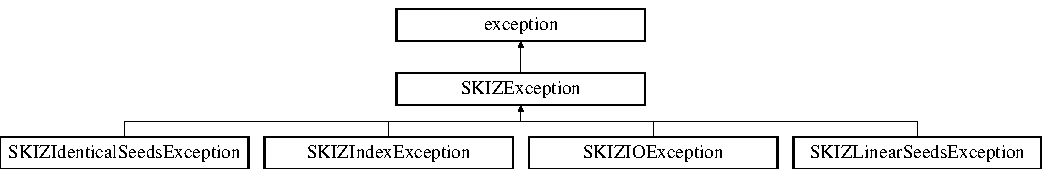
\includegraphics[height=1.816216cm]{classSKIZException}
\end{center}
\end{figure}
\subsection*{Public Member Functions}
\begin{DoxyCompactItemize}
\item 
\mbox{\Hypertarget{classSKIZException_a30a47c59e9fd4ea93441c9029c4068d9}\label{classSKIZException_a30a47c59e9fd4ea93441c9029c4068d9}} 
\mbox{\hyperlink{classSKIZException_a30a47c59e9fd4ea93441c9029c4068d9}{S\+K\+I\+Z\+Exception}} (const std\+::string s)
\begin{DoxyCompactList}\small\item\em Constructor takes string as argument which is stored in msg. \end{DoxyCompactList}\item 
\mbox{\Hypertarget{classSKIZException_ac1b8f1ba8ae87ce018c645a1a67b6d34}\label{classSKIZException_ac1b8f1ba8ae87ce018c645a1a67b6d34}} 
virtual \mbox{\hyperlink{classSKIZException_ac1b8f1ba8ae87ce018c645a1a67b6d34}{$\sim$\+S\+K\+I\+Z\+Exception}} ()  throw ()
\begin{DoxyCompactList}\small\item\em Destructor. \end{DoxyCompactList}\item 
\mbox{\Hypertarget{classSKIZException_a55c36f650f02f283215679ad070dd54b}\label{classSKIZException_a55c36f650f02f283215679ad070dd54b}} 
const char $\ast$ \mbox{\hyperlink{classSKIZException_a55c36f650f02f283215679ad070dd54b}{what}} ()
\begin{DoxyCompactList}\small\item\em Extract message stored in msg. \end{DoxyCompactList}\end{DoxyCompactItemize}


\subsection{Detailed Description}
Parent class for all S\+K\+IZ exceptions. 


\begin{DoxyParams}{Parameters}
{\em s} & Message to be given when thrown \\
\hline
\end{DoxyParams}


The documentation for this class was generated from the following files\+:\begin{DoxyCompactItemize}
\item 
src/\mbox{\hyperlink{skizException_8h}{skiz\+Exception.\+h}}\item 
src/\mbox{\hyperlink{skizException_8cpp}{skiz\+Exception.\+cpp}}\end{DoxyCompactItemize}

\hypertarget{classSKIZIdenticalSeedsException}{}\section{S\+K\+I\+Z\+Identical\+Seeds\+Exception Class Reference}
\label{classSKIZIdenticalSeedsException}\index{S\+K\+I\+Z\+Identical\+Seeds\+Exception@{S\+K\+I\+Z\+Identical\+Seeds\+Exception}}


Thrown if add\+Seed is given a seed to add to Voronoi diagram where one already exists.  




{\ttfamily \#include $<$skiz\+Exception.\+h$>$}

Inheritance diagram for S\+K\+I\+Z\+Identical\+Seeds\+Exception\+:\begin{figure}[H]
\begin{center}
\leavevmode
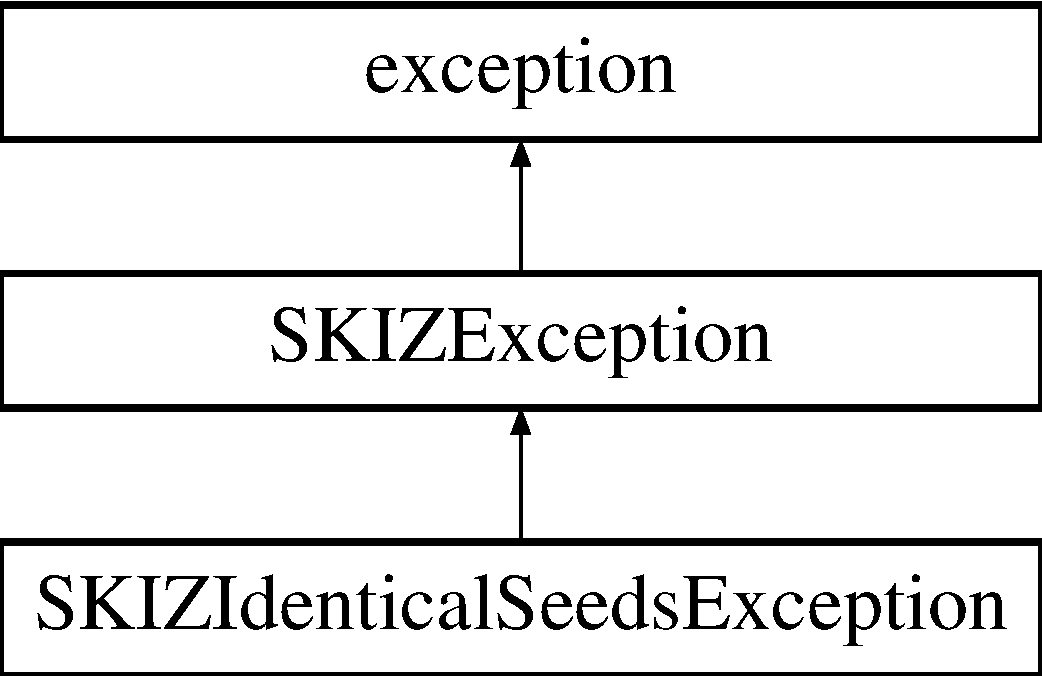
\includegraphics[height=3.000000cm]{classSKIZIdenticalSeedsException}
\end{center}
\end{figure}
\subsection*{Public Member Functions}
\begin{DoxyCompactItemize}
\item 
\mbox{\Hypertarget{classSKIZIdenticalSeedsException_a776554e938f17373b9de355c81eb78e3}\label{classSKIZIdenticalSeedsException_a776554e938f17373b9de355c81eb78e3}} 
\mbox{\hyperlink{classSKIZIdenticalSeedsException_a776554e938f17373b9de355c81eb78e3}{S\+K\+I\+Z\+Identical\+Seeds\+Exception}} (const std\+::string s)
\begin{DoxyCompactList}\small\item\em Constructor takes string as argument which is stored in msg. \end{DoxyCompactList}\item 
\mbox{\Hypertarget{classSKIZIdenticalSeedsException_addce88717ce4fe89ef5d431e7fdff84b}\label{classSKIZIdenticalSeedsException_addce88717ce4fe89ef5d431e7fdff84b}} 
virtual \mbox{\hyperlink{classSKIZIdenticalSeedsException_addce88717ce4fe89ef5d431e7fdff84b}{$\sim$\+S\+K\+I\+Z\+Identical\+Seeds\+Exception}} ()  throw ()
\begin{DoxyCompactList}\small\item\em Destructor. \end{DoxyCompactList}\item 
\mbox{\Hypertarget{classSKIZIdenticalSeedsException_a1edd2deac7bafc875e21c67d114494ae}\label{classSKIZIdenticalSeedsException_a1edd2deac7bafc875e21c67d114494ae}} 
const char $\ast$ \mbox{\hyperlink{classSKIZIdenticalSeedsException_a1edd2deac7bafc875e21c67d114494ae}{what}} ()
\begin{DoxyCompactList}\small\item\em Extract message stored in msg. \end{DoxyCompactList}\end{DoxyCompactItemize}


\subsection{Detailed Description}
Thrown if add\+Seed is given a seed to add to Voronoi diagram where one already exists. 


\begin{DoxyParams}{Parameters}
{\em s} & Message to be given when thrown \\
\hline
\end{DoxyParams}


The documentation for this class was generated from the following files\+:\begin{DoxyCompactItemize}
\item 
src/\mbox{\hyperlink{skizException_8h}{skiz\+Exception.\+h}}\item 
src/\mbox{\hyperlink{skizException_8cpp}{skiz\+Exception.\+cpp}}\end{DoxyCompactItemize}

\hypertarget{classSKIZIndexException}{}\section{S\+K\+I\+Z\+Index\+Exception Class Reference}
\label{classSKIZIndexException}\index{S\+K\+I\+Z\+Index\+Exception@{S\+K\+I\+Z\+Index\+Exception}}


Thrown when trying to access a non-\/existent entry in a std\+::vector or std\+::map.  




{\ttfamily \#include $<$skiz\+Exception.\+h$>$}

Inheritance diagram for S\+K\+I\+Z\+Index\+Exception\+:\begin{figure}[H]
\begin{center}
\leavevmode
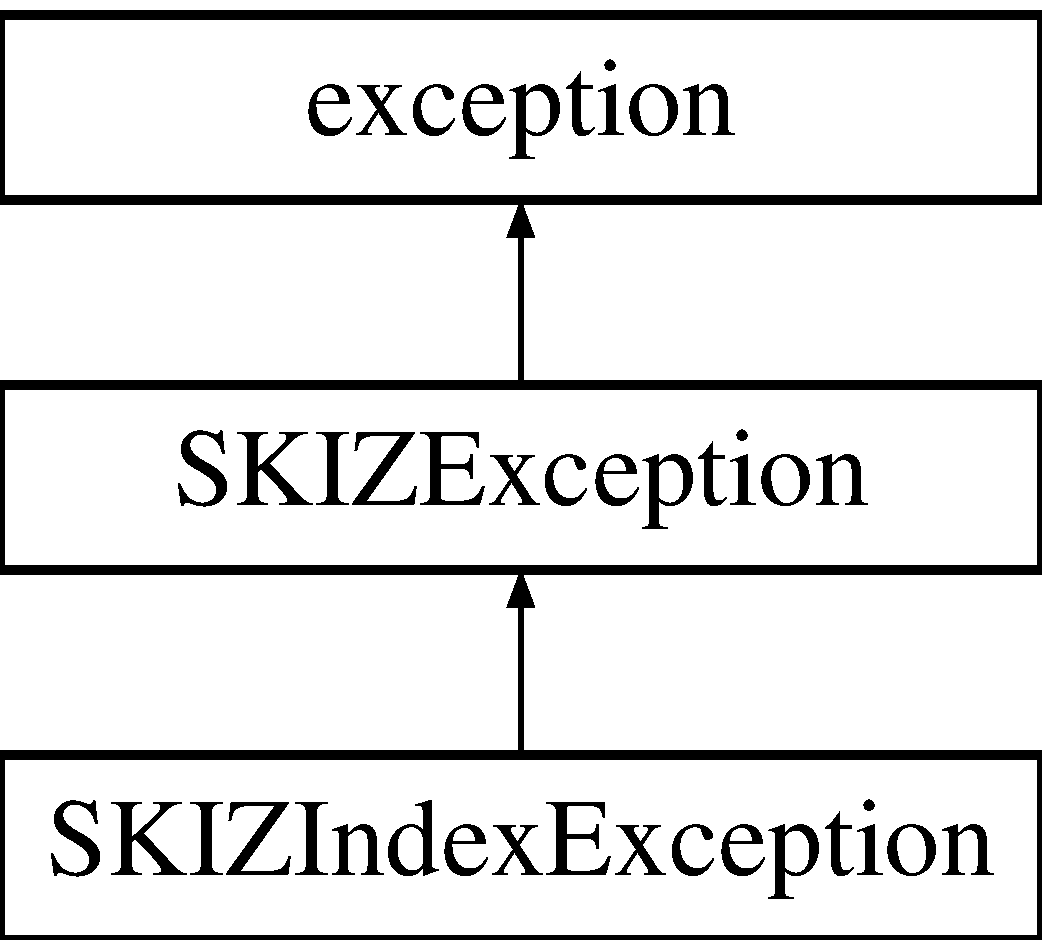
\includegraphics[height=3.000000cm]{classSKIZIndexException}
\end{center}
\end{figure}
\subsection*{Public Member Functions}
\begin{DoxyCompactItemize}
\item 
\mbox{\Hypertarget{classSKIZIndexException_abd89a7895a20077dbb514271c6455f75}\label{classSKIZIndexException_abd89a7895a20077dbb514271c6455f75}} 
\mbox{\hyperlink{classSKIZIndexException_abd89a7895a20077dbb514271c6455f75}{S\+K\+I\+Z\+Index\+Exception}} (const std\+::string s)
\begin{DoxyCompactList}\small\item\em Constructor takes string as argument which is stored in msg. \end{DoxyCompactList}\item 
\mbox{\Hypertarget{classSKIZIndexException_ad41e9aa637c94d9e559f84333c6fafb5}\label{classSKIZIndexException_ad41e9aa637c94d9e559f84333c6fafb5}} 
virtual \mbox{\hyperlink{classSKIZIndexException_ad41e9aa637c94d9e559f84333c6fafb5}{$\sim$\+S\+K\+I\+Z\+Index\+Exception}} ()  throw ()
\begin{DoxyCompactList}\small\item\em Destructor. \end{DoxyCompactList}\item 
\mbox{\Hypertarget{classSKIZIndexException_a9f02457a3301bf0618023b25f8d79007}\label{classSKIZIndexException_a9f02457a3301bf0618023b25f8d79007}} 
const char $\ast$ {\bfseries what} ()
\end{DoxyCompactItemize}


\subsection{Detailed Description}
Thrown when trying to access a non-\/existent entry in a std\+::vector or std\+::map. 


\begin{DoxyParams}{Parameters}
{\em s} & Message to be given when thrown \\
\hline
\end{DoxyParams}


The documentation for this class was generated from the following files\+:\begin{DoxyCompactItemize}
\item 
\mbox{\hyperlink{skizException_8h}{skiz\+Exception.\+h}}\item 
\mbox{\hyperlink{skizException_8cpp}{skiz\+Exception.\+cpp}}\end{DoxyCompactItemize}

\hypertarget{classSKIZIOException}{}\section{S\+K\+I\+Z\+I\+O\+Exception Class Reference}
\label{classSKIZIOException}\index{S\+K\+I\+Z\+I\+O\+Exception@{S\+K\+I\+Z\+I\+O\+Exception}}


Thrown in case of failure to open a file for reading or writing.  




{\ttfamily \#include $<$skiz\+Exception.\+h$>$}

Inheritance diagram for S\+K\+I\+Z\+I\+O\+Exception\+:\begin{figure}[H]
\begin{center}
\leavevmode
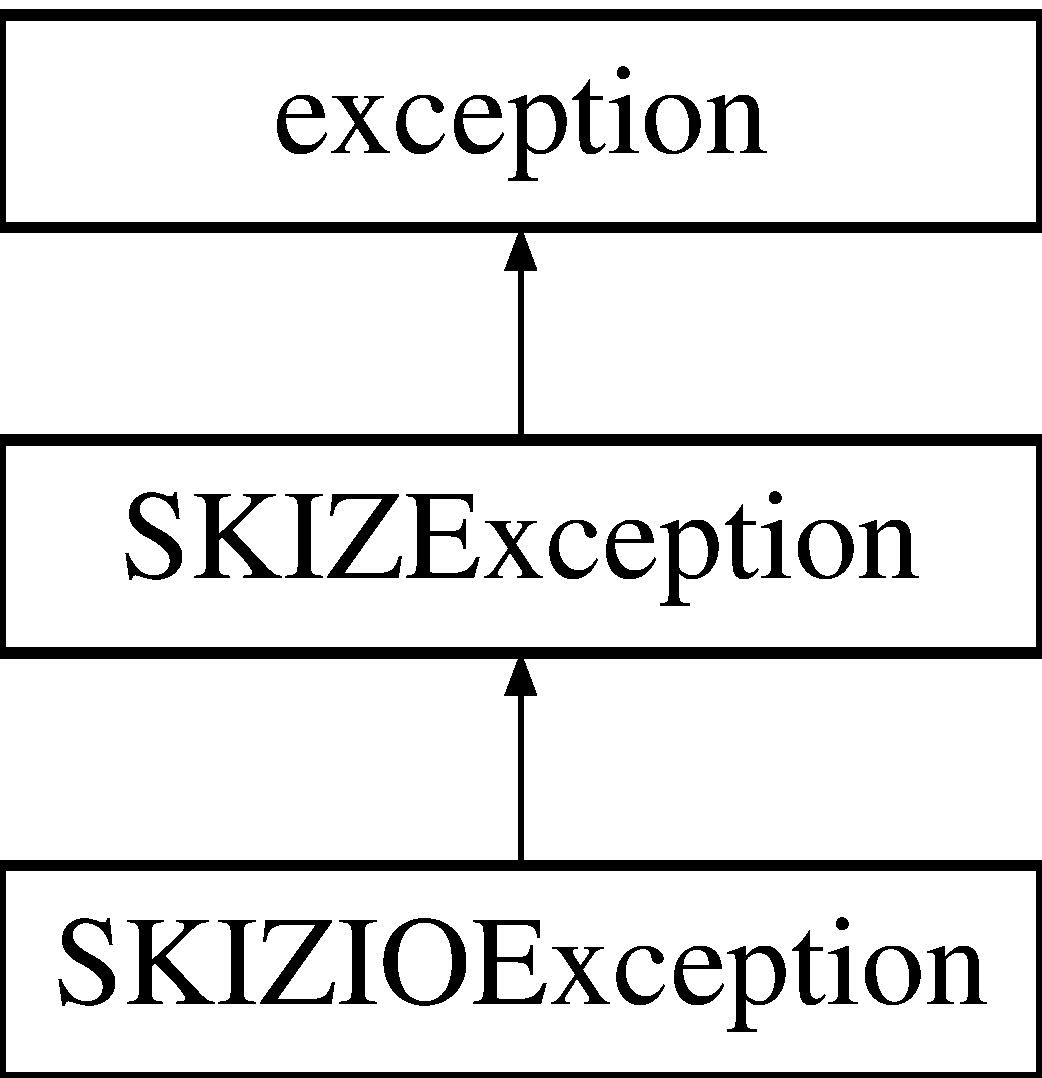
\includegraphics[height=3.000000cm]{classSKIZIOException}
\end{center}
\end{figure}
\subsection*{Public Member Functions}
\begin{DoxyCompactItemize}
\item 
\mbox{\Hypertarget{classSKIZIOException_a9f25dbc11996a8755965923611cce128}\label{classSKIZIOException_a9f25dbc11996a8755965923611cce128}} 
\mbox{\hyperlink{classSKIZIOException_a9f25dbc11996a8755965923611cce128}{S\+K\+I\+Z\+I\+O\+Exception}} (const std\+::string s)
\begin{DoxyCompactList}\small\item\em Constructor takes string as argument which is stored in msg. \end{DoxyCompactList}\item 
\mbox{\Hypertarget{classSKIZIOException_af331baab993a6666a5f6509a332510b3}\label{classSKIZIOException_af331baab993a6666a5f6509a332510b3}} 
virtual \mbox{\hyperlink{classSKIZIOException_af331baab993a6666a5f6509a332510b3}{$\sim$\+S\+K\+I\+Z\+I\+O\+Exception}} ()  throw ()
\begin{DoxyCompactList}\small\item\em Destructor. \end{DoxyCompactList}\item 
\mbox{\Hypertarget{classSKIZIOException_a9c1c40e5e47cb51fb0fb3803cdae4a76}\label{classSKIZIOException_a9c1c40e5e47cb51fb0fb3803cdae4a76}} 
const char $\ast$ \mbox{\hyperlink{classSKIZIOException_a9c1c40e5e47cb51fb0fb3803cdae4a76}{what}} ()
\begin{DoxyCompactList}\small\item\em Extract message stored in msg. \end{DoxyCompactList}\end{DoxyCompactItemize}


\subsection{Detailed Description}
Thrown in case of failure to open a file for reading or writing. 


\begin{DoxyParams}{Parameters}
{\em s} & Message to be given when thrown \\
\hline
\end{DoxyParams}


The documentation for this class was generated from the following files\+:\begin{DoxyCompactItemize}
\item 
\mbox{\hyperlink{skizException_8h}{skiz\+Exception.\+h}}\item 
\mbox{\hyperlink{skizException_8cpp}{skiz\+Exception.\+cpp}}\end{DoxyCompactItemize}

\hypertarget{classSKIZLinearSeedsException}{}\section{S\+K\+I\+Z\+Linear\+Seeds\+Exception Class Reference}
\label{classSKIZLinearSeedsException}\index{S\+K\+I\+Z\+Linear\+Seeds\+Exception@{S\+K\+I\+Z\+Linear\+Seeds\+Exception}}


Thrown by circumcentre if input coordinates form a line.  




{\ttfamily \#include $<$skiz\+Exception.\+h$>$}

Inheritance diagram for S\+K\+I\+Z\+Linear\+Seeds\+Exception\+:\begin{figure}[H]
\begin{center}
\leavevmode
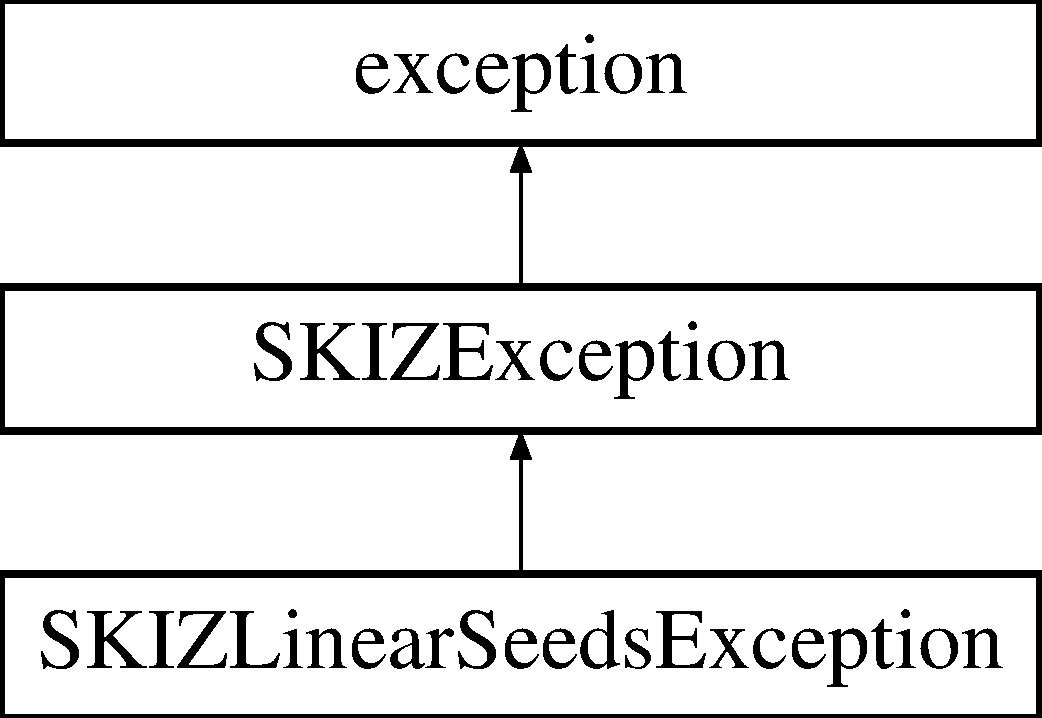
\includegraphics[height=3.000000cm]{classSKIZLinearSeedsException}
\end{center}
\end{figure}
\subsection*{Public Member Functions}
\begin{DoxyCompactItemize}
\item 
\mbox{\Hypertarget{classSKIZLinearSeedsException_a11607556ca04d52a2d2c35c06fad3f6b}\label{classSKIZLinearSeedsException_a11607556ca04d52a2d2c35c06fad3f6b}} 
\mbox{\hyperlink{classSKIZLinearSeedsException_a11607556ca04d52a2d2c35c06fad3f6b}{S\+K\+I\+Z\+Linear\+Seeds\+Exception}} (const std\+::string s)
\begin{DoxyCompactList}\small\item\em Constructor takes string as argument which is stored in msg. \end{DoxyCompactList}\item 
\mbox{\Hypertarget{classSKIZLinearSeedsException_a8482d8d51517e183205757fd4855107b}\label{classSKIZLinearSeedsException_a8482d8d51517e183205757fd4855107b}} 
virtual \mbox{\hyperlink{classSKIZLinearSeedsException_a8482d8d51517e183205757fd4855107b}{$\sim$\+S\+K\+I\+Z\+Linear\+Seeds\+Exception}} ()  throw ()
\begin{DoxyCompactList}\small\item\em Destructor. \end{DoxyCompactList}\item 
\mbox{\Hypertarget{classSKIZLinearSeedsException_a4d187b93ce4261b7303ab75e23e06e30}\label{classSKIZLinearSeedsException_a4d187b93ce4261b7303ab75e23e06e30}} 
const char $\ast$ \mbox{\hyperlink{classSKIZLinearSeedsException_a4d187b93ce4261b7303ab75e23e06e30}{what}} ()
\begin{DoxyCompactList}\small\item\em Extract message stored in msg. \end{DoxyCompactList}\end{DoxyCompactItemize}


\subsection{Detailed Description}
Thrown by circumcentre if input coordinates form a line. 


\begin{DoxyParams}{Parameters}
{\em s} & Message to be given when thrown \\
\hline
\end{DoxyParams}


The documentation for this class was generated from the following files\+:\begin{DoxyCompactItemize}
\item 
src/\mbox{\hyperlink{skizException_8h}{skiz\+Exception.\+h}}\item 
src/\mbox{\hyperlink{skizException_8cpp}{skiz\+Exception.\+cpp}}\end{DoxyCompactItemize}

\hypertarget{structV__struct}{}\section{V\+\_\+struct Struct Reference}
\label{structV__struct}\index{V\+\_\+struct@{V\+\_\+struct}}


as defined in \mbox{[}1\mbox{]}, Section 3 (Vk).  




{\ttfamily \#include $<$vd.\+h$>$}

\subsection*{Data Fields}
\begin{DoxyCompactItemize}
\item 
\mbox{\hyperlink{typedefs_8h_a9fa28c1f74e909474857584f5c7b0088}{Mat}} \mbox{\hyperlink{structV__struct_a56d1655953ba5bee519bd62d992abfff}{lam}}
\item 
\mbox{\hyperlink{typedefs_8h_a9fa28c1f74e909474857584f5c7b0088}{Mat}} \mbox{\hyperlink{structV__struct_aa78c83185af94c1df09f59a689881cd9}{v}}
\end{DoxyCompactItemize}


\subsection{Detailed Description}
as defined in \mbox{[}1\mbox{]}, Section 3 (Vk). 

\subsection{Field Documentation}
\mbox{\Hypertarget{structV__struct_a56d1655953ba5bee519bd62d992abfff}\label{structV__struct_a56d1655953ba5bee519bd62d992abfff}} 
\index{V\+\_\+struct@{V\+\_\+struct}!lam@{lam}}
\index{lam@{lam}!V\+\_\+struct@{V\+\_\+struct}}
\subsubsection{\texorpdfstring{lam}{lam}}
{\footnotesize\ttfamily \mbox{\hyperlink{typedefs_8h_a9fa28c1f74e909474857584f5c7b0088}{Mat}} V\+\_\+struct\+::lam}

\mbox{\Hypertarget{structV__struct_aa78c83185af94c1df09f59a689881cd9}\label{structV__struct_aa78c83185af94c1df09f59a689881cd9}} 
\index{V\+\_\+struct@{V\+\_\+struct}!v@{v}}
\index{v@{v}!V\+\_\+struct@{V\+\_\+struct}}
\subsubsection{\texorpdfstring{v}{v}}
{\footnotesize\ttfamily \mbox{\hyperlink{typedefs_8h_a9fa28c1f74e909474857584f5c7b0088}{Mat}} V\+\_\+struct\+::v}



The documentation for this struct was generated from the following file\+:\begin{DoxyCompactItemize}
\item 
src/\mbox{\hyperlink{vd_8h}{vd.\+h}}\end{DoxyCompactItemize}

\hypertarget{classvd}{}\section{vd Class Reference}
\label{classvd}\index{vd@{vd}}
\subsection*{Public Member Functions}
\begin{DoxyCompactItemize}
\item 
\mbox{\Hypertarget{classvd_a062d265bd642352d6f7e8cc8685ed7a8}\label{classvd_a062d265bd642352d6f7e8cc8685ed7a8}} 
void {\bfseries set\+Vk} (\mbox{\hyperlink{structV__struct}{V\+\_\+struct}} val)
\item 
\mbox{\Hypertarget{classvd_a85ee3a096c181f76d15f4b7fcf137fe7}\label{classvd_a85ee3a096c181f76d15f4b7fcf137fe7}} 
void {\bfseries setW} (\mbox{\hyperlink{structW__struct}{W\+\_\+struct}} val)
\item 
\mbox{\Hypertarget{classvd_a36a19417f43a4316d0172a8ce3476e8e}\label{classvd_a36a19417f43a4316d0172a8ce3476e8e}} 
void {\bfseries setS} (\mbox{\hyperlink{structS__struct}{S\+\_\+struct}} val)
\item 
\mbox{\Hypertarget{classvd_ae13e9e465d08425218bd8f85ce420c05}\label{classvd_ae13e9e465d08425218bd8f85ce420c05}} 
void {\bfseries set\+Lam} (\mbox{\hyperlink{aux_8h_aa1fe91b8cd36c618282eb0d548690c4c}{Mat}} new\+Lam)
\item 
\mbox{\Hypertarget{classvd_a33e792915ebd0295a3475fe686b41ee9}\label{classvd_a33e792915ebd0295a3475fe686b41ee9}} 
void {\bfseries setV} (\mbox{\hyperlink{aux_8h_aa1fe91b8cd36c618282eb0d548690c4c}{Mat}} newV)
\item 
\mbox{\Hypertarget{classvd_a772224a2d677a8f8a5cf86d27b5795c8}\label{classvd_a772224a2d677a8f8a5cf86d27b5795c8}} 
void {\bfseries set\+Lam\+By\+Idx} (unsigned int i, unsigned int j, real val)
\item 
\mbox{\Hypertarget{classvd_a53e18ea21521a36ab65a1de417466a9b}\label{classvd_a53e18ea21521a36ab65a1de417466a9b}} 
void {\bfseries set\+V\+By\+Idx} (unsigned int i, unsigned int j, real val)
\item 
\mbox{\Hypertarget{classvd_a739318bbb45d4facfcc1899c71b91720}\label{classvd_a739318bbb45d4facfcc1899c71b91720}} 
void {\bfseries set\+Seeds} (\mbox{\hyperlink{aux_8h_aa1fe91b8cd36c618282eb0d548690c4c}{Mat}} s)
\item 
\mbox{\Hypertarget{classvd_a579df0c885a43bb876449889bbcba6cb}\label{classvd_a579df0c885a43bb876449889bbcba6cb}} 
void {\bfseries set\+Px} (\mbox{\hyperlink{aux_8h_aa1fe91b8cd36c618282eb0d548690c4c}{Mat}} x)
\item 
\mbox{\Hypertarget{classvd_a8314de29eacf72f10afee2c67b0c9819}\label{classvd_a8314de29eacf72f10afee2c67b0c9819}} 
void {\bfseries set\+Py} (\mbox{\hyperlink{aux_8h_aa1fe91b8cd36c618282eb0d548690c4c}{Mat}} y)
\item 
\mbox{\Hypertarget{classvd_a7c692a97b49c4596c4ec1bc0a129b516}\label{classvd_a7c692a97b49c4596c4ec1bc0a129b516}} 
void {\bfseries setK} (real val)
\item 
\mbox{\Hypertarget{classvd_afb492f7d32ff2a4d54bd531d57d66a1a}\label{classvd_afb492f7d32ff2a4d54bd531d57d66a1a}} 
void {\bfseries set\+Sx} (std\+::map$<$ real, real $>$ val)
\item 
\mbox{\Hypertarget{classvd_af103a45c726643e96f69be4363ad2409}\label{classvd_af103a45c726643e96f69be4363ad2409}} 
void {\bfseries set\+Sy} (std\+::map$<$ real, real $>$ val)
\item 
\mbox{\Hypertarget{classvd_a42dc1ab4c7033c49c0b3716d461ad2ef}\label{classvd_a42dc1ab4c7033c49c0b3716d461ad2ef}} 
void {\bfseries set\+Sk} (std\+::map$<$ real, real $>$ val)
\item 
\mbox{\Hypertarget{classvd_a28b1a96051112e13734bd09fdfa0e165}\label{classvd_a28b1a96051112e13734bd09fdfa0e165}} 
void {\bfseries set\+Sx\+By\+Idx} (unsigned int idx, real val)
\item 
\mbox{\Hypertarget{classvd_abb229381c39157015dad7cdfd095b434}\label{classvd_abb229381c39157015dad7cdfd095b434}} 
void {\bfseries set\+Sy\+By\+Idx} (unsigned int idx, real val)
\item 
\mbox{\Hypertarget{classvd_a777ef30414be47a33432358750802d0a}\label{classvd_a777ef30414be47a33432358750802d0a}} 
void {\bfseries set\+Sk\+By\+Idx} (unsigned int idx, real val)
\item 
\mbox{\Hypertarget{classvd_aa1a3d9448f6ff6f8076b15c9e9a63d7e}\label{classvd_aa1a3d9448f6ff6f8076b15c9e9a63d7e}} 
void {\bfseries set\+Nk} (std\+::map$<$ real, \mbox{\hyperlink{aux_8h_ac0a1a538b45426e056715d1f59f854ab}{Real\+Vec}} $>$ val)
\item 
\mbox{\Hypertarget{classvd_a769ad1fef725d8e644c4634fe7d5a559}\label{classvd_a769ad1fef725d8e644c4634fe7d5a559}} 
void {\bfseries set\+Nk\+By\+Value} (unsigned int idx, \mbox{\hyperlink{aux_8h_ac0a1a538b45426e056715d1f59f854ab}{Real\+Vec}} val)
\item 
\mbox{\Hypertarget{classvd_a59c1f5756af7de9cc7a0089221cbd5b7}\label{classvd_a59c1f5756af7de9cc7a0089221cbd5b7}} 
void {\bfseries incrementK} ()
\item 
\mbox{\Hypertarget{classvd_a090bebdbbff36888934c870daf3dcb36}\label{classvd_a090bebdbbff36888934c870daf3dcb36}} 
\mbox{\hyperlink{structV__struct}{V\+\_\+struct}} {\bfseries get\+Vk} () const
\item 
\mbox{\Hypertarget{classvd_ab4d0d9ea76cedf1a6825b62c9ec2d118}\label{classvd_ab4d0d9ea76cedf1a6825b62c9ec2d118}} 
\mbox{\hyperlink{structW__struct}{W\+\_\+struct}} {\bfseries getW} () const
\item 
\mbox{\Hypertarget{classvd_a6b1b73738e720c8ffa2351841c44eabb}\label{classvd_a6b1b73738e720c8ffa2351841c44eabb}} 
\mbox{\hyperlink{structS__struct}{S\+\_\+struct}} {\bfseries getS} () const
\item 
\mbox{\Hypertarget{classvd_a37c4ab12669eb276fe7fa4a610310345}\label{classvd_a37c4ab12669eb276fe7fa4a610310345}} 
\mbox{\hyperlink{aux_8h_aa1fe91b8cd36c618282eb0d548690c4c}{Mat}} {\bfseries get\+Lam} () const
\item 
\mbox{\Hypertarget{classvd_aad4ea5c045b8380f83b0490af2fee0fa}\label{classvd_aad4ea5c045b8380f83b0490af2fee0fa}} 
\mbox{\hyperlink{aux_8h_aa1fe91b8cd36c618282eb0d548690c4c}{Mat}} {\bfseries getV} () const
\item 
\mbox{\Hypertarget{classvd_a1f2400a9f98f649367239f942e3035e8}\label{classvd_a1f2400a9f98f649367239f942e3035e8}} 
real {\bfseries get\+Lam\+By\+Idx} (unsigned int i, unsigned int j) const
\item 
\mbox{\Hypertarget{classvd_af5dbddcd8db66e57e17c4ca65f0a1a0c}\label{classvd_af5dbddcd8db66e57e17c4ca65f0a1a0c}} 
real {\bfseries get\+V\+By\+Idx} (unsigned int i, unsigned int j) const
\item 
\mbox{\Hypertarget{classvd_a82f353c594c3c6b24f6077398f059d3a}\label{classvd_a82f353c594c3c6b24f6077398f059d3a}} 
\mbox{\hyperlink{aux_8h_aa1fe91b8cd36c618282eb0d548690c4c}{Mat}} {\bfseries get\+Seeds} () const
\item 
\mbox{\Hypertarget{classvd_aeba6d318016c8f8b9537ce4c0314f8cd}\label{classvd_aeba6d318016c8f8b9537ce4c0314f8cd}} 
\mbox{\hyperlink{aux_8h_aa1fe91b8cd36c618282eb0d548690c4c}{Mat}} {\bfseries get\+Px} () const
\item 
\mbox{\Hypertarget{classvd_a9738711704b1d03cdbe027b1976cb0c6}\label{classvd_a9738711704b1d03cdbe027b1976cb0c6}} 
\mbox{\hyperlink{aux_8h_aa1fe91b8cd36c618282eb0d548690c4c}{Mat}} {\bfseries get\+Py} () const
\item 
\mbox{\Hypertarget{classvd_a624f53ae4a7012f267111359e9245f81}\label{classvd_a624f53ae4a7012f267111359e9245f81}} 
real {\bfseries getK} () const
\item 
\mbox{\Hypertarget{classvd_a1a1634d6906eb0af4d877c2af3292ca7}\label{classvd_a1a1634d6906eb0af4d877c2af3292ca7}} 
real {\bfseries get\+Nr} () const
\item 
\mbox{\Hypertarget{classvd_ab0de0a5b8929ed7a7bb6ca902a462dd4}\label{classvd_ab0de0a5b8929ed7a7bb6ca902a462dd4}} 
real {\bfseries get\+Nc} () const
\item 
\mbox{\Hypertarget{classvd_a58ca0f2dcf014942947f48d311c20d02}\label{classvd_a58ca0f2dcf014942947f48d311c20d02}} 
std\+::map$<$ real, real $>$ {\bfseries get\+Sx} () const
\item 
\mbox{\Hypertarget{classvd_a47295ea4089a6798c40288bac1656c91}\label{classvd_a47295ea4089a6798c40288bac1656c91}} 
std\+::map$<$ real, real $>$ {\bfseries get\+Sy} () const
\item 
\mbox{\Hypertarget{classvd_af16eada5667f835ecce3cdc2956098c9}\label{classvd_af16eada5667f835ecce3cdc2956098c9}} 
std\+::map$<$ real, real $>$ {\bfseries get\+Sk} () const
\item 
\mbox{\Hypertarget{classvd_af4a6bc90137ebfe5242fbcd36524bf5b}\label{classvd_af4a6bc90137ebfe5242fbcd36524bf5b}} 
std\+::map$<$ real, \mbox{\hyperlink{aux_8h_ac0a1a538b45426e056715d1f59f854ab}{Real\+Vec}} $>$ {\bfseries get\+Nk} () const
\item 
\mbox{\Hypertarget{classvd_a765c16ee377a2a0f9651d555edd3a158}\label{classvd_a765c16ee377a2a0f9651d555edd3a158}} 
{\bfseries vd} (real rows, real cols)
\end{DoxyCompactItemize}
\subsection*{Public Attributes}
\begin{DoxyCompactItemize}
\item 
\mbox{\Hypertarget{classvd_aca8bd9fa239b6fadf3b3a25e5c17557e}\label{classvd_aca8bd9fa239b6fadf3b3a25e5c17557e}} 
\mbox{\hyperlink{structV__struct}{V\+\_\+struct}} {\bfseries Vk}
\item 
\mbox{\Hypertarget{classvd_ab23d33e6c11c46ad3302a874a4726542}\label{classvd_ab23d33e6c11c46ad3302a874a4726542}} 
\mbox{\hyperlink{structW__struct}{W\+\_\+struct}} {\bfseries W}
\item 
\mbox{\Hypertarget{classvd_a047f87d1fc7c8fea5f6cc4f6d4f228fa}\label{classvd_a047f87d1fc7c8fea5f6cc4f6d4f228fa}} 
\mbox{\hyperlink{structS__struct}{S\+\_\+struct}} {\bfseries S}
\item 
\mbox{\Hypertarget{classvd_a989a61c00de8a517c1093aba6f7d1b22}\label{classvd_a989a61c00de8a517c1093aba6f7d1b22}} 
real {\bfseries nc}
\item 
\mbox{\Hypertarget{classvd_a04271075413d6082dad757da678d0181}\label{classvd_a04271075413d6082dad757da678d0181}} 
real {\bfseries nr}
\item 
\mbox{\Hypertarget{classvd_a0cbfe9c7ca1e17901cc232d57352f200}\label{classvd_a0cbfe9c7ca1e17901cc232d57352f200}} 
real {\bfseries k}
\item 
\mbox{\Hypertarget{classvd_aebb5bd18cba152453d0c74134c233d0e}\label{classvd_aebb5bd18cba152453d0c74134c233d0e}} 
\mbox{\hyperlink{aux_8h_aa1fe91b8cd36c618282eb0d548690c4c}{Mat}} {\bfseries seeds}
\item 
\mbox{\Hypertarget{classvd_afc15550440d0c6bc61d917f4ac75aa75}\label{classvd_afc15550440d0c6bc61d917f4ac75aa75}} 
\mbox{\hyperlink{aux_8h_aa1fe91b8cd36c618282eb0d548690c4c}{Mat}} {\bfseries px}
\item 
\mbox{\Hypertarget{classvd_a71b266194d117645ce8a3aeee98499f9}\label{classvd_a71b266194d117645ce8a3aeee98499f9}} 
\mbox{\hyperlink{aux_8h_aa1fe91b8cd36c618282eb0d548690c4c}{Mat}} {\bfseries py}
\item 
\mbox{\Hypertarget{classvd_a2c1599932c0909f80abd6cf7601940f6}\label{classvd_a2c1599932c0909f80abd6cf7601940f6}} 
std\+::map$<$ real, real $>$ {\bfseries Sx}
\item 
\mbox{\Hypertarget{classvd_abfa4f5d8305394eed7e36fabbb65e782}\label{classvd_abfa4f5d8305394eed7e36fabbb65e782}} 
std\+::map$<$ real, real $>$ {\bfseries Sy}
\item 
\mbox{\Hypertarget{classvd_a8b0e7202fac9d8411a0b3d1e6960bf5e}\label{classvd_a8b0e7202fac9d8411a0b3d1e6960bf5e}} 
std\+::map$<$ real, real $>$ {\bfseries Sk}
\item 
\mbox{\Hypertarget{classvd_a417f0bd0c1c54c7d927352df356134b6}\label{classvd_a417f0bd0c1c54c7d927352df356134b6}} 
std\+::map$<$ real, \mbox{\hyperlink{aux_8h_ac0a1a538b45426e056715d1f59f854ab}{Real\+Vec}} $>$ {\bfseries Nk}
\end{DoxyCompactItemize}


The documentation for this class was generated from the following files\+:\begin{DoxyCompactItemize}
\item 
vd.\+h\item 
vd.\+cpp\end{DoxyCompactItemize}

\hypertarget{structW__struct}{}\section{W\+\_\+struct Struct Reference}
\label{structW__struct}\index{W\+\_\+struct@{W\+\_\+struct}}


as defined in \mbox{[}1\mbox{]}, Section 2.\+2. Only for use with V\+O\+I\+SE algorithm matlab interface. Unused but here for consistency.  




{\ttfamily \#include $<$vd.\+h$>$}

\subsection*{Public Attributes}
\begin{DoxyCompactItemize}
\item 
\mbox{\Hypertarget{structW__struct_a7c0ed763a5701a0787361a68cad4aec4}\label{structW__struct_a7c0ed763a5701a0787361a68cad4aec4}} 
real {\bfseries xm}
\item 
\mbox{\Hypertarget{structW__struct_a69290893bf3fc1a9bf0ff987a9e25320}\label{structW__struct_a69290893bf3fc1a9bf0ff987a9e25320}} 
real {\bfseries ym}
\item 
\mbox{\Hypertarget{structW__struct_a20e12df215aaa6a737a15b05e6102093}\label{structW__struct_a20e12df215aaa6a737a15b05e6102093}} 
real {\bfseries xM}
\item 
\mbox{\Hypertarget{structW__struct_a10de004bf31c6563ad0a55116a96cd8d}\label{structW__struct_a10de004bf31c6563ad0a55116a96cd8d}} 
real {\bfseries yM}
\end{DoxyCompactItemize}


\subsection{Detailed Description}
as defined in \mbox{[}1\mbox{]}, Section 2.\+2. Only for use with V\+O\+I\+SE algorithm matlab interface. Unused but here for consistency. 

The documentation for this struct was generated from the following file\+:\begin{DoxyCompactItemize}
\item 
\mbox{\hyperlink{vd_8h}{vd.\+h}}\end{DoxyCompactItemize}

\chapter{File Documentation}
\hypertarget{addSeed_8cpp}{}\section{add\+Seed.\+cpp File Reference}
\label{addSeed_8cpp}\index{add\+Seed.\+cpp@{add\+Seed.\+cpp}}


Adds seed to Voronoi diagram.  


{\ttfamily \#include \char`\"{}add\+Seed.\+h\char`\"{}}\newline
{\ttfamily \#include \char`\"{}skiz\+Exception.\+h\char`\"{}}\newline
{\ttfamily \#include \char`\"{}N\+S\+Star.\+h\char`\"{}}\newline
{\ttfamily \#include \char`\"{}point\+In\+Region.\+h\char`\"{}}\newline
{\ttfamily \#include \char`\"{}get\+Region.\+h\char`\"{}}\newline
{\ttfamily \#include \char`\"{}aux.\+h\char`\"{}}\newline
{\ttfamily \#include \char`\"{}typedefs.\+cpp\char`\"{}}\newline
{\ttfamily \#include $<$iostream$>$}\newline
\subsection*{Macros}
\begin{DoxyCompactItemize}
\item 
\mbox{\Hypertarget{addSeed_8cpp_a12c2040f25d8e3a7b9e1c2024c618cb6}\label{addSeed_8cpp_a12c2040f25d8e3a7b9e1c2024c618cb6}} 
\#define {\bfseries I\+NF}~std\+::numeric\+\_\+limits$<$\mbox{\hyperlink{typedefs_8cpp_a58a0c7cf2501f4492da833421be92547}{real}}$>$\+::infinity()
\end{DoxyCompactItemize}
\subsection*{Functions}
\begin{DoxyCompactItemize}
\item 
\mbox{\Hypertarget{addSeed_8cpp_aed9f982f10e3e3fb1c9c0903274b3728}\label{addSeed_8cpp_aed9f982f10e3e3fb1c9c0903274b3728}} 
bool {\bfseries add\+Seed} (\mbox{\hyperlink{classvd}{vd}} \&VD, \mbox{\hyperlink{typedefs_8cpp_a58a0c7cf2501f4492da833421be92547}{real}} s1, \mbox{\hyperlink{typedefs_8cpp_a58a0c7cf2501f4492da833421be92547}{real}} s2)
\end{DoxyCompactItemize}


\subsection{Detailed Description}
Adds seed to Voronoi diagram. 


\hypertarget{addSeed_8h}{}\section{src/add\+Seed.h File Reference}
\label{addSeed_8h}\index{src/add\+Seed.\+h@{src/add\+Seed.\+h}}
{\ttfamily \#include \char`\"{}vd.\+h\char`\"{}}\newline
\subsection*{Functions}
\begin{DoxyCompactItemize}
\item 
void \mbox{\hyperlink{addSeed_8h_a6d39c734e0cb94bd35d1b7f2b147f245}{add\+Seed}} (\mbox{\hyperlink{classvd}{vd}} \&\mbox{\hyperlink{testRemoveSeedCheckV_8cpp_a17edf6f20961d07c702ee68bb30d9bf3}{VD}}, \mbox{\hyperlink{typedefs_8h_a58a0c7cf2501f4492da833421be92547}{real}} s1, \mbox{\hyperlink{typedefs_8h_a58a0c7cf2501f4492da833421be92547}{real}} s2)
\end{DoxyCompactItemize}


\subsection{Detailed Description}

\hypertarget{circumcentre_8h}{}\section{src/aux-\/functions/circumcentre.h File Reference}
\label{circumcentre_8h}\index{src/aux-\/functions/circumcentre.\+h@{src/aux-\/functions/circumcentre.\+h}}


Finds the cirumcentre of the triangle formed by three given points (templated). Header only for templating/linking reasons.  


\subsection*{Functions}
\begin{DoxyCompactItemize}
\item 
{\footnotesize template$<$class T1 , class T2 , class T3 , class T4 , class T5 , class T6 $>$ }\\std\+::array$<$ \mbox{\hyperlink{typedefs_8cpp_a58a0c7cf2501f4492da833421be92547}{real}}, 2 $>$ {\bfseries circumcentre} (const T1 \&ax, const T2 \&ay, const T3 \&bx, const T4 \&by, const T5 \&cx, const T6 \&cy)
\end{DoxyCompactItemize}


\subsection{Detailed Description}
Finds the cirumcentre of the triangle formed by three given points (templated). Header only for templating/linking reasons. 


\hypertarget{inVector_8h}{}\section{src/aux-\/functions/in\+Vector.h File Reference}
\label{inVector_8h}\index{src/aux-\/functions/in\+Vector.\+h@{src/aux-\/functions/in\+Vector.\+h}}


Checks whether item exists within a vector. Header only for templating/linking reasons.  


{\ttfamily \#include $<$vector$>$}\newline
{\ttfamily \#include \char`\"{}../typedefs.\+cpp\char`\"{}}\newline
\subsection*{Functions}
\begin{DoxyCompactItemize}
\item 
{\footnotesize template$<$class T1 , class T2 $>$ }\\bool {\bfseries in\+Vector} (const std\+::vector$<$ T1 $>$ \&vec, const T2 \&item)
\end{DoxyCompactItemize}


\subsection{Detailed Description}
Checks whether item exists within a vector. Header only for templating/linking reasons. 


\hypertarget{readMatrix_8cpp}{}\section{src/aux-\/functions/read\+Matrix.cpp File Reference}
\label{readMatrix_8cpp}\index{src/aux-\/functions/read\+Matrix.\+cpp@{src/aux-\/functions/read\+Matrix.\+cpp}}


Reads matrix from ascii-\/formatted files generated by Matlab\textquotesingle{}s \textquotesingle{}save\textquotesingle{} function.  


{\ttfamily \#include \char`\"{}../typedefs.\+h\char`\"{}}\newline
{\ttfamily \#include \char`\"{}read\+Matrix.\+h\char`\"{}}\newline
{\ttfamily \#include $<$string$>$}\newline
{\ttfamily \#include $<$fstream$>$}\newline
{\ttfamily \#include $<$iostream$>$}\newline
\subsection*{Functions}
\begin{DoxyCompactItemize}
\item 
\mbox{\Hypertarget{readMatrix_8cpp_aeb74858e69439fc90841ccf4e124d9fa}\label{readMatrix_8cpp_aeb74858e69439fc90841ccf4e124d9fa}} 
\mbox{\hyperlink{typedefs_8h_a9fa28c1f74e909474857584f5c7b0088}{Mat}} {\bfseries read\+Matrix} (std\+::string filename)
\end{DoxyCompactItemize}


\subsection{Detailed Description}
Reads matrix from ascii-\/formatted files generated by Matlab\textquotesingle{}s \textquotesingle{}save\textquotesingle{} function. 


\hypertarget{readSeeds_8cpp}{}\section{src/aux-\/functions/read\+Seeds.cpp File Reference}
\label{readSeeds_8cpp}\index{src/aux-\/functions/read\+Seeds.\+cpp@{src/aux-\/functions/read\+Seeds.\+cpp}}


Reads seed coordinates from ascii-\/formatted files generated by Matlab\textquotesingle{}s \textquotesingle{}save\textquotesingle{} function.  


{\ttfamily \#include \char`\"{}read\+Seeds.\+h\char`\"{}}\newline
{\ttfamily \#include $<$string$>$}\newline
{\ttfamily \#include $<$fstream$>$}\newline
\subsection*{Functions}
\begin{DoxyCompactItemize}
\item 
std\+::vector$<$ \mbox{\hyperlink{typedefs_8h_a84b6d9a0fbb45e01ad4a3aa5667f2992}{Real\+Vec}} $>$ \mbox{\hyperlink{readSeeds_8cpp_ad85b04f26adf16a2034600271b5cbcb3}{read\+Seeds}} (std\+::string filename)
\end{DoxyCompactItemize}


\subsection{Detailed Description}
Reads seed coordinates from ascii-\/formatted files generated by Matlab\textquotesingle{}s \textquotesingle{}save\textquotesingle{} function. 


\hypertarget{sqDist_8h}{}\section{src/aux-\/functions/sq\+Dist.h File Reference}
\label{sqDist_8h}\index{src/aux-\/functions/sq\+Dist.\+h@{src/aux-\/functions/sq\+Dist.\+h}}


Finds the squared difference between two points (templated). Header only for templating/linking reasons.  


{\ttfamily \#include \char`\"{}../typedefs.\+cpp\char`\"{}}\newline
\subsection*{Functions}
\begin{DoxyCompactItemize}
\item 
{\footnotesize template$<$class T1 , class T2 , class T3 , class T4 $>$ }\\\mbox{\hyperlink{typedefs_8cpp_a58a0c7cf2501f4492da833421be92547}{real}} {\bfseries sq\+Dist} (const T1 \&p1, const T2 \&p2, const T3 \&q1, const T4 \&q2)
\end{DoxyCompactItemize}


\subsection{Detailed Description}
Finds the squared difference between two points (templated). Header only for templating/linking reasons. 


\hypertarget{updateDict_8h}{}\section{src/aux-\/functions/update\+Dict.h File Reference}
\label{updateDict_8h}\index{src/aux-\/functions/update\+Dict.\+h@{src/aux-\/functions/update\+Dict.\+h}}


Routine for adding to the vector in a dictionary of vectors only if the item does not already exist (templated). Header only for templating/linking reasons.  


{\ttfamily \#include $<$vector$>$}\newline
{\ttfamily \#include $<$map$>$}\newline
\subsection*{Functions}
\begin{DoxyCompactItemize}
\item 
{\footnotesize template$<$class T1 , class T2 , class T3 , class T4 $>$ }\\void \mbox{\hyperlink{updateDict_8h_ae4e5cf796db8a46b879fec6b4b9418af}{update\+Dict}} (std\+::map$<$ T1, std\+::vector$<$ T2 $>$$>$ \&d, const T3 \&key, const T4 \&value)
\end{DoxyCompactItemize}


\subsection{Detailed Description}
Routine for adding to the vector in a dictionary of vectors only if the item does not already exist (templated). Header only for templating/linking reasons. 


\hypertarget{getRegion_8cpp}{}\section{get\+Region.\+cpp File Reference}
\label{getRegion_8cpp}\index{get\+Region.\+cpp@{get\+Region.\+cpp}}


Finds the voronoi region R(s) of a seed s.  


{\ttfamily \#include $<$eigen3/\+Eigen/\+Dense$>$}\newline
{\ttfamily \#include $<$math.\+h$>$}\newline
{\ttfamily \#include \char`\"{}get\+Region.\+h\char`\"{}}\newline
\subsection*{Functions}
\begin{DoxyCompactItemize}
\item 
\mbox{\Hypertarget{getRegion_8cpp_a9a53c64cf58a7df70dd9c7477feda3ce}\label{getRegion_8cpp_a9a53c64cf58a7df70dd9c7477feda3ce}} 
\mbox{\hyperlink{aux_8h_aa1fe91b8cd36c618282eb0d548690c4c}{Mat}} {\bfseries get\+Region} (const \mbox{\hyperlink{classvd}{vd}} \&VD, const real \&s)
\end{DoxyCompactItemize}


\subsection{Detailed Description}
Finds the voronoi region R(s) of a seed s. 


\hypertarget{getRegion_8h}{}\section{get\+Region.\+h File Reference}
\label{getRegion_8h}\index{get\+Region.\+h@{get\+Region.\+h}}
{\ttfamily \#include $<$eigen3/\+Eigen/\+Dense$>$}\newline
{\ttfamily \#include \char`\"{}vd.\+h\char`\"{}}\newline
{\ttfamily \#include \char`\"{}typedefs.\+cpp\char`\"{}}\newline
\subsection*{Functions}
\begin{DoxyCompactItemize}
\item 
\mbox{\Hypertarget{getRegion_8h_a9a53c64cf58a7df70dd9c7477feda3ce}\label{getRegion_8h_a9a53c64cf58a7df70dd9c7477feda3ce}} 
\mbox{\hyperlink{aux_8h_aa1fe91b8cd36c618282eb0d548690c4c}{Mat}} {\bfseries get\+Region} (const \mbox{\hyperlink{classvd}{vd}} \&VD, const real \&s)
\end{DoxyCompactItemize}


\subsection{Detailed Description}

\hypertarget{addSeedToVD_8cpp}{}\section{src/mex/add\+Seed\+To\+VD.cpp File Reference}
\label{addSeedToVD_8cpp}\index{src/mex/add\+Seed\+To\+V\+D.\+cpp@{src/mex/add\+Seed\+To\+V\+D.\+cpp}}


This is a M\+EX function. It should only be compiled by the compile\+M\+E\+X.\+m matlab script. Adds single seeds to Voronoi diagram.  


{\ttfamily \#include $<$eigen3/\+Eigen/\+Dense$>$}\newline
{\ttfamily \#include $<$map$>$}\newline
{\ttfamily \#include \char`\"{}../vd.\+h\char`\"{}}\newline
{\ttfamily \#include \char`\"{}../add\+Seed.\+h\char`\"{}}\newline
{\ttfamily \#include \char`\"{}../skiz\+Exception.\+h\char`\"{}}\newline
{\ttfamily \#include \char`\"{}grab\+V\+D.\+h\char`\"{}}\newline
{\ttfamily \#include \char`\"{}push\+V\+D.\+h\char`\"{}}\newline
\subsection*{Functions}
\begin{DoxyCompactItemize}
\item 
\mbox{\Hypertarget{addSeedToVD_8cpp_a6a215cbfde54f82a3ce599228fc3fce5}\label{addSeedToVD_8cpp_a6a215cbfde54f82a3ce599228fc3fce5}} 
void {\bfseries mex\+Function} (int nlhs, mx\+Array $\ast$plhs\mbox{[}$\,$\mbox{]}, int nrhs, const mx\+Array $\ast$prhs\mbox{[}$\,$\mbox{]})
\end{DoxyCompactItemize}


\subsection{Detailed Description}
This is a M\+EX function. It should only be compiled by the compile\+M\+E\+X.\+m matlab script. Adds single seeds to Voronoi diagram. 


\hypertarget{addSeedToVDBatch_8cpp}{}\section{src/mex/add\+Seed\+To\+V\+D\+Batch.cpp File Reference}
\label{addSeedToVDBatch_8cpp}\index{src/mex/add\+Seed\+To\+V\+D\+Batch.\+cpp@{src/mex/add\+Seed\+To\+V\+D\+Batch.\+cpp}}


This is a M\+EX function. It should only be compiled by the compile\+M\+E\+X.\+m matlab script.  


{\ttfamily \#include $<$eigen3/\+Eigen/\+Dense$>$}\newline
{\ttfamily \#include $<$map$>$}\newline
{\ttfamily \#include \char`\"{}../vd.\+h\char`\"{}}\newline
{\ttfamily \#include \char`\"{}../add\+Seed.\+h\char`\"{}}\newline
{\ttfamily \#include \char`\"{}../skiz\+Exception.\+h\char`\"{}}\newline
{\ttfamily \#include \char`\"{}grab\+V\+D.\+h\char`\"{}}\newline
{\ttfamily \#include \char`\"{}push\+V\+D.\+h\char`\"{}}\newline
\subsection*{Functions}
\begin{DoxyCompactItemize}
\item 
\mbox{\Hypertarget{addSeedToVDBatch_8cpp_a6a215cbfde54f82a3ce599228fc3fce5}\label{addSeedToVDBatch_8cpp_a6a215cbfde54f82a3ce599228fc3fce5}} 
void {\bfseries mex\+Function} (int nlhs, mx\+Array $\ast$plhs\mbox{[}$\,$\mbox{]}, int nrhs, const mx\+Array $\ast$prhs\mbox{[}$\,$\mbox{]})
\end{DoxyCompactItemize}


\subsection{Detailed Description}
This is a M\+EX function. It should only be compiled by the compile\+M\+E\+X.\+m matlab script. 


\hypertarget{getCentroidSeedBatch_8cpp}{}\section{src/mex/get\+Centroid\+Seed\+Batch.cpp File Reference}
\label{getCentroidSeedBatch_8cpp}\index{src/mex/get\+Centroid\+Seed\+Batch.\+cpp@{src/mex/get\+Centroid\+Seed\+Batch.\+cpp}}


This is a M\+EX function. It should only be compiled by the compile\+M\+E\+X.\+m matlab script. Uses one of six metrics (mean, median, standard deviation, range, normalised range, number of pixels) to evaluate the merit function of a Voronoi region.  


{\ttfamily \#include $<$eigen3/\+Eigen/\+Dense$>$}\newline
{\ttfamily \#include \char`\"{}../vd.\+h\char`\"{}}\newline
{\ttfamily \#include \char`\"{}../get\+Region.\+h\char`\"{}}\newline
{\ttfamily \#include \char`\"{}../typedefs.\+cpp\char`\"{}}\newline
{\ttfamily \#include \char`\"{}grab\+V\+D.\+h\char`\"{}}\newline
{\ttfamily \#include \char`\"{}grab\+W.\+h\char`\"{}}\newline
\subsection*{Functions}
\begin{DoxyCompactItemize}
\item 
void \mbox{\hyperlink{getCentroidSeedBatch_8cpp_a6a215cbfde54f82a3ce599228fc3fce5}{mex\+Function}} (int nlhs, mx\+Array $\ast$plhs\mbox{[}$\,$\mbox{]}, int nrhs, const mx\+Array $\ast$prhs\mbox{[}$\,$\mbox{]})
\begin{DoxyCompactList}\small\item\em This is a M\+EX function. As such, the inputs and outputs are constricted to the following\+: \end{DoxyCompactList}\end{DoxyCompactItemize}


\subsection{Detailed Description}
This is a M\+EX function. It should only be compiled by the compile\+M\+E\+X.\+m matlab script. Uses one of six metrics (mean, median, standard deviation, range, normalised range, number of pixels) to evaluate the merit function of a Voronoi region. 


\hypertarget{getVDOp_8cpp}{}\section{src/mex/get\+V\+D\+Op.cpp File Reference}
\label{getVDOp_8cpp}\index{src/mex/get\+V\+D\+Op.\+cpp@{src/mex/get\+V\+D\+Op.\+cpp}}


This is a M\+EX function. It should only be compiled by the compile\+M\+E\+X.\+m matlab script. Uses one of six metrics (mean, median, standard deviation, range, normalised range, number of pixels) to evaluate the merit function of a Voronoi region.  


{\ttfamily \#include $<$eigen3/\+Eigen/\+Dense$>$}\newline
{\ttfamily \#include $<$map$>$}\newline
{\ttfamily \#include $<$functional$>$}\newline
{\ttfamily \#include $<$string$>$}\newline
{\ttfamily \#include \char`\"{}../vd.\+h\char`\"{}}\newline
{\ttfamily \#include \char`\"{}../skiz\+Exception.\+h\char`\"{}}\newline
{\ttfamily \#include \char`\"{}../get\+Region.\+h\char`\"{}}\newline
{\ttfamily \#include \char`\"{}../aux-\/functions/metrics.\+h\char`\"{}}\newline
{\ttfamily \#include \char`\"{}grab\+V\+D.\+h\char`\"{}}\newline
{\ttfamily \#include \char`\"{}push\+V\+D.\+h\char`\"{}}\newline
{\ttfamily \#include \char`\"{}grab\+W.\+h\char`\"{}}\newline
\subsection*{Functions}
\begin{DoxyCompactItemize}
\item 
void \mbox{\hyperlink{getVDOp_8cpp_a6a215cbfde54f82a3ce599228fc3fce5}{mex\+Function}} (int nlhs, mx\+Array $\ast$plhs\mbox{[}$\,$\mbox{]}, int nrhs, const mx\+Array $\ast$prhs\mbox{[}$\,$\mbox{]})
\begin{DoxyCompactList}\small\item\em This is a M\+EX function, and as such the inputs and outputs are constricted to the following\+: \end{DoxyCompactList}\end{DoxyCompactItemize}


\subsection{Detailed Description}
This is a M\+EX function. It should only be compiled by the compile\+M\+E\+X.\+m matlab script. Uses one of six metrics (mean, median, standard deviation, range, normalised range, number of pixels) to evaluate the merit function of a Voronoi region. 



\subsection{Function Documentation}
\mbox{\Hypertarget{getVDOp_8cpp_a6a215cbfde54f82a3ce599228fc3fce5}\label{getVDOp_8cpp_a6a215cbfde54f82a3ce599228fc3fce5}} 
\index{get\+V\+D\+Op.\+cpp@{get\+V\+D\+Op.\+cpp}!mex\+Function@{mex\+Function}}
\index{mex\+Function@{mex\+Function}!get\+V\+D\+Op.\+cpp@{get\+V\+D\+Op.\+cpp}}
\subsubsection{\texorpdfstring{mex\+Function()}{mexFunction()}}
{\footnotesize\ttfamily void mex\+Function (\begin{DoxyParamCaption}\item[{int}]{nlhs,  }\item[{mx\+Array $\ast$}]{plhs\mbox{[}$\,$\mbox{]},  }\item[{int}]{nrhs,  }\item[{const mx\+Array $\ast$}]{prhs\mbox{[}$\,$\mbox{]} }\end{DoxyParamCaption})}



This is a M\+EX function, and as such the inputs and outputs are constricted to the following\+: 


\begin{DoxyParams}{Parameters}
{\em nlhs} & Number of outputs \\
\hline
{\em plhs} & Pointer to outputs \\
\hline
{\em nrhs} & Number of inputs \\
\hline
{\em prhs} & Pointer to inputs\\
\hline
\end{DoxyParams}
In Matlab, this corresponds to the following parameters and outputs\+: 
\begin{DoxyParams}{Parameters}
{\em VD} & Voronoi diagram struct \\
\hline
{\em W} & Matrix of pixel values \\
\hline
{\em metric\+ID} & Key from 1-\/6 indicating which metric to use\+: (1) Median (2) Mean (3) Range (4) Square root of the number of pixels (5) Normalised range (6) Standard deviation \\
\hline
{\em mult} & (For metric\+ID = 5 and 6 only) Multiplier of each pixel. For metric\+ID = 5, coefficient is 1/mult. For metric\+ID = 6, coefficient is equal to mult. \\
\hline
\end{DoxyParams}
\begin{DoxyReturn}{Returns}
Sop Vector of metric value for each Voronoi region 

Wop Matrix of metric values for each pixel. All pixels in same voronoi region have same Wop value. Pixels equidistant from two or more closest seeds (with $ \nu_{ij} $ = 1) have Wop $_{ij} $ = NaN, as per the Matlab implementation. 
\end{DoxyReturn}

\hypertarget{grabVD_8cpp}{}\section{src/mex/grab\+VD.cpp File Reference}
\label{grabVD_8cpp}\index{src/mex/grab\+V\+D.\+cpp@{src/mex/grab\+V\+D.\+cpp}}


This is a M\+EX function. It should only be compiled by the compile\+M\+E\+X.\+m matlab script. Allocates memory and populates vd object with data from matlab VD struct. Only for use with Matlab mex compiler.  


{\ttfamily \#include \char`\"{}mex\+Includes.\+h\char`\"{}}\newline
\subsection*{Functions}
\begin{DoxyCompactItemize}
\item 
\mbox{\Hypertarget{grabVD_8cpp_aed17a6085a5808aa18fd3c0deac0725d}\label{grabVD_8cpp_aed17a6085a5808aa18fd3c0deac0725d}} 
\mbox{\hyperlink{classvd}{vd}} {\bfseries grab\+VD} (const mx\+Array $\ast$prhs\mbox{[}$\,$\mbox{]}, const \mbox{\hyperlink{typedefs_8cpp_a8ad23e2333787a214e20a58a284a5a60}{uint32}} field)
\end{DoxyCompactItemize}


\subsection{Detailed Description}
This is a M\+EX function. It should only be compiled by the compile\+M\+E\+X.\+m matlab script. Allocates memory and populates vd object with data from matlab VD struct. Only for use with Matlab mex compiler. 


\hypertarget{grabVD_8h}{}\section{grab\+V\+D.\+h File Reference}
\label{grabVD_8h}\index{grab\+V\+D.\+h@{grab\+V\+D.\+h}}
{\ttfamily \#include \char`\"{}vd.\+h\char`\"{}}\newline
\subsection*{Functions}
\begin{DoxyCompactItemize}
\item 
\mbox{\Hypertarget{grabVD_8h_ab8fe56ea31d841b1fa3af459ef58cf94}\label{grabVD_8h_ab8fe56ea31d841b1fa3af459ef58cf94}} 
\mbox{\hyperlink{classvd}{vd}} {\bfseries grab\+VD} (const mx\+Array $\ast$prhs\mbox{[}$\,$\mbox{]})
\end{DoxyCompactItemize}


\subsection{Detailed Description}

\hypertarget{grabW_8cpp}{}\section{src/mex/grabW.cpp File Reference}
\label{grabW_8cpp}\index{src/mex/grab\+W.\+cpp@{src/mex/grab\+W.\+cpp}}


This is a requirement for a M\+EX function. It should only be compiled by the compile\+M\+E\+X.\+m Matlab script. Gets params.\+W matrix from VD Matlab struct.  


{\ttfamily \#include \char`\"{}grab\+W.\+h\char`\"{}}\newline
\subsection*{Functions}
\begin{DoxyCompactItemize}
\item 
\mbox{\Hypertarget{grabW_8cpp_afabbbfade012bae6f28ba4bf8a9643d7}\label{grabW_8cpp_afabbbfade012bae6f28ba4bf8a9643d7}} 
\mbox{\hyperlink{typedefs_8cpp_a9fa28c1f74e909474857584f5c7b0088}{Mat}} {\bfseries grabW} (const mx\+Array $\ast$prhs\mbox{[}$\,$\mbox{]}, const \mbox{\hyperlink{typedefs_8cpp_a8ad23e2333787a214e20a58a284a5a60}{uint32}} field)
\end{DoxyCompactItemize}


\subsection{Detailed Description}
This is a requirement for a M\+EX function. It should only be compiled by the compile\+M\+E\+X.\+m Matlab script. Gets params.\+W matrix from VD Matlab struct. 


\hypertarget{pushVD_8cpp}{}\section{src/mex/push\+VD.cpp File Reference}
\label{pushVD_8cpp}\index{src/mex/push\+V\+D.\+cpp@{src/mex/push\+V\+D.\+cpp}}


This is a requirement for a M\+EX function. It should only be compiled by the compile\+M\+E\+X.\+m matlab script. Allocates memory and populates Matlab struct with data from vd object. Only for use with Matlab mex compiler.  


{\ttfamily \#include \char`\"{}mex\+Includes.\+h\char`\"{}}\newline
\subsection*{Functions}
\begin{DoxyCompactItemize}
\item 
\mbox{\Hypertarget{pushVD_8cpp_ac94a6cb8acb6660e46a6da5f00fe9e9c}\label{pushVD_8cpp_ac94a6cb8acb6660e46a6da5f00fe9e9c}} 
void {\bfseries push\+VD} (\mbox{\hyperlink{classvd}{vd}} output\+VD, mx\+Array $\ast$plhs\mbox{[}$\,$\mbox{]})
\end{DoxyCompactItemize}


\subsection{Detailed Description}
This is a requirement for a M\+EX function. It should only be compiled by the compile\+M\+E\+X.\+m matlab script. Allocates memory and populates Matlab struct with data from vd object. Only for use with Matlab mex compiler. 


\hypertarget{pushVD_8h}{}\section{push\+V\+D.\+h File Reference}
\label{pushVD_8h}\index{push\+V\+D.\+h@{push\+V\+D.\+h}}
{\ttfamily \#include \char`\"{}vd.\+h\char`\"{}}\newline
\subsection*{Functions}
\begin{DoxyCompactItemize}
\item 
\mbox{\Hypertarget{pushVD_8h_ac94a6cb8acb6660e46a6da5f00fe9e9c}\label{pushVD_8h_ac94a6cb8acb6660e46a6da5f00fe9e9c}} 
void {\bfseries push\+VD} (\mbox{\hyperlink{classvd}{vd}} output\+VD, mx\+Array $\ast$plhs\mbox{[}$\,$\mbox{]})
\end{DoxyCompactItemize}


\subsection{Detailed Description}

\hypertarget{NSStar_8cpp}{}\section{src/\+N\+S\+Star.cpp File Reference}
\label{NSStar_8cpp}\index{src/\+N\+S\+Star.\+cpp@{src/\+N\+S\+Star.\+cpp}}


Finds neighbouring Voronoi regions for new seeds.  


{\ttfamily \#include $<$map$>$}\newline
{\ttfamily \#include \char`\"{}N\+S\+Star.\+h\char`\"{}}\newline
{\ttfamily \#include \char`\"{}point\+In\+Region.\+h\char`\"{}}\newline
{\ttfamily \#include \char`\"{}skiz\+Exception.\+h\char`\"{}}\newline
{\ttfamily \#include \char`\"{}aux-\/functions/in\+Vector.\+h\char`\"{}}\newline
{\ttfamily \#include \char`\"{}aux-\/functions/circumcentre.\+h\char`\"{}}\newline
\subsection*{Functions}
\begin{DoxyCompactItemize}
\item 
\mbox{\Hypertarget{NSStar_8cpp_a08c5bf29a9c4aadfa72d49fd80a49ab0}\label{NSStar_8cpp_a08c5bf29a9c4aadfa72d49fd80a49ab0}} 
\mbox{\hyperlink{typedefs_8cpp_a84b6d9a0fbb45e01ad4a3aa5667f2992}{Real\+Vec}} {\bfseries ns\+Star} (const \mbox{\hyperlink{classvd}{vd}} \&VD)
\end{DoxyCompactItemize}


\subsection{Detailed Description}
Finds neighbouring Voronoi regions for new seeds. 


\hypertarget{NSStar_8h}{}\section{N\+S\+Star.\+h File Reference}
\label{NSStar_8h}\index{N\+S\+Star.\+h@{N\+S\+Star.\+h}}
{\ttfamily \#include $<$vector$>$}\newline
{\ttfamily \#include \char`\"{}vd.\+h\char`\"{}}\newline
\subsection*{Functions}
\begin{DoxyCompactItemize}
\item 
\mbox{\Hypertarget{NSStar_8h_a08c5bf29a9c4aadfa72d49fd80a49ab0}\label{NSStar_8h_a08c5bf29a9c4aadfa72d49fd80a49ab0}} 
Real\+Vec {\bfseries ns\+Star} (const \mbox{\hyperlink{classvd}{vd}} \&VD)
\end{DoxyCompactItemize}


\subsection{Detailed Description}

\hypertarget{pointInRegion_8cpp}{}\section{point\+In\+Region.\+cpp File Reference}
\label{pointInRegion_8cpp}\index{point\+In\+Region.\+cpp@{point\+In\+Region.\+cpp}}


Checks whether a point is within region C(s, A) according to the definition 2.\+5 in the S\+K\+IZ paper \mbox{[} D\+OI\+: 10.\+1109/34.\+625128 \mbox{]}.  


{\ttfamily \#include \char`\"{}point\+In\+Region.\+h\char`\"{}}\newline
{\ttfamily \#include \char`\"{}skiz\+Exception.\+h\char`\"{}}\newline
\subsection*{Macros}
\begin{DoxyCompactItemize}
\item 
\mbox{\Hypertarget{pointInRegion_8cpp_a179dcf7e366d81e4229117de7ba5bc71}\label{pointInRegion_8cpp_a179dcf7e366d81e4229117de7ba5bc71}} 
\#define {\bfseries P\+O\+I\+N\+T\+I\+N\+R\+E\+G\+I\+O\+N\+\_\+H}
\item 
\mbox{\Hypertarget{pointInRegion_8cpp_a598e1edca6bb53498b755e10b8533847}\label{pointInRegion_8cpp_a598e1edca6bb53498b755e10b8533847}} 
\#define {\bfseries S\+K\+I\+Z\+\_\+\+S\+K\+I\+Z\+E\+X\+C\+E\+P\+T\+I\+O\+N\+\_\+H}
\item 
\mbox{\Hypertarget{pointInRegion_8cpp_a12c2040f25d8e3a7b9e1c2024c618cb6}\label{pointInRegion_8cpp_a12c2040f25d8e3a7b9e1c2024c618cb6}} 
\#define {\bfseries I\+NF}~std\+::numeric\+\_\+limits$<$real$>$\+::infinity()
\end{DoxyCompactItemize}
\subsection*{Functions}
\begin{DoxyCompactItemize}
\item 
bool \mbox{\hyperlink{pointInRegion_8cpp_aa0cec93776a85c9bbf81ee69390d4bbd}{point\+In\+Region}} (const \mbox{\hyperlink{classvd}{vd}} \&VD, std\+::array$<$ real, 2 $>$ pt, real s, Real\+Vec A)
\begin{DoxyCompactList}\small\item\em Checks whether a point is within region C(s, A) according to the definition 2.\+5 in the S\+K\+IZ paper \mbox{[} D\+OI\+: 10.\+1109/34.\+625128 \mbox{]}. \end{DoxyCompactList}\end{DoxyCompactItemize}


\subsection{Detailed Description}
Checks whether a point is within region C(s, A) according to the definition 2.\+5 in the S\+K\+IZ paper \mbox{[} D\+OI\+: 10.\+1109/34.\+625128 \mbox{]}. 



\subsection{Function Documentation}
\mbox{\Hypertarget{pointInRegion_8cpp_aa0cec93776a85c9bbf81ee69390d4bbd}\label{pointInRegion_8cpp_aa0cec93776a85c9bbf81ee69390d4bbd}} 
\index{point\+In\+Region.\+cpp@{point\+In\+Region.\+cpp}!point\+In\+Region@{point\+In\+Region}}
\index{point\+In\+Region@{point\+In\+Region}!point\+In\+Region.\+cpp@{point\+In\+Region.\+cpp}}
\subsubsection{\texorpdfstring{point\+In\+Region()}{pointInRegion()}}
{\footnotesize\ttfamily point\+In\+Region (\begin{DoxyParamCaption}\item[{const \mbox{\hyperlink{classvd}{vd}} \&}]{VD,  }\item[{std\+::array$<$ real, 2 $>$}]{pt,  }\item[{real}]{s,  }\item[{Real\+Vec}]{A }\end{DoxyParamCaption})}



Checks whether a point is within region C(s, A) according to the definition 2.\+5 in the S\+K\+IZ paper \mbox{[} D\+OI\+: 10.\+1109/34.\+625128 \mbox{]}. 


\begin{DoxyParams}{Parameters}
{\em vd} & Voronoi Diagram \\
\hline
{\em pt} & x and y coordinates of point to check \\
\hline
{\em s} & Index of seed which defines the region being checked \\
\hline
{\em A} & Vector of seeds which together form half-\/planes that make up C(s, A) \\
\hline
\end{DoxyParams}
\begin{DoxyReturn}{Returns}
true\+: Point is in C(s, A) 

false\+: Point is not in C(s, A) 
\end{DoxyReturn}

\hypertarget{pointInRegion_8h}{}\section{point\+In\+Region.\+h File Reference}
\label{pointInRegion_8h}\index{point\+In\+Region.\+h@{point\+In\+Region.\+h}}


Checks whether a point is within region C(s, A) according to the definition 2.\+5 in the S\+K\+IZ paper \mbox{[} D\+OI\+: 10.\+1109/34.\+625128 \mbox{]}.  


{\ttfamily \#include $<$vector$>$}\newline
{\ttfamily \#include \char`\"{}vd.\+h\char`\"{}}\newline
{\ttfamily \#include \char`\"{}typedefs.\+cpp\char`\"{}}\newline
\subsection*{Functions}
\begin{DoxyCompactItemize}
\item 
bool \mbox{\hyperlink{pointInRegion_8h_acbc5d3411a9380422cb9ac4f2723f5a7}{point\+In\+Region}} (const \mbox{\hyperlink{classvd}{vd}} \&VD, std\+::array$<$ real, 2 $>$ pt, real s, \mbox{\hyperlink{aux_8h_ac0a1a538b45426e056715d1f59f854ab}{Real\+Vec}} A)
\begin{DoxyCompactList}\small\item\em Checks whether a point is within region C(s, A) according to the definition 2.\+5 in the S\+K\+IZ paper \mbox{[} D\+OI\+: 10.\+1109/34.\+625128 \mbox{]}. \end{DoxyCompactList}\end{DoxyCompactItemize}


\subsection{Detailed Description}
Checks whether a point is within region C(s, A) according to the definition 2.\+5 in the S\+K\+IZ paper \mbox{[} D\+OI\+: 10.\+1109/34.\+625128 \mbox{]}. 



\subsection{Function Documentation}
\mbox{\Hypertarget{pointInRegion_8h_acbc5d3411a9380422cb9ac4f2723f5a7}\label{pointInRegion_8h_acbc5d3411a9380422cb9ac4f2723f5a7}} 
\index{point\+In\+Region.\+h@{point\+In\+Region.\+h}!point\+In\+Region@{point\+In\+Region}}
\index{point\+In\+Region@{point\+In\+Region}!point\+In\+Region.\+h@{point\+In\+Region.\+h}}
\subsubsection{\texorpdfstring{point\+In\+Region()}{pointInRegion()}}
{\footnotesize\ttfamily bool point\+In\+Region (\begin{DoxyParamCaption}\item[{const \mbox{\hyperlink{classvd}{vd}} \&}]{VD,  }\item[{std\+::array$<$ real, 2 $>$}]{pt,  }\item[{real}]{s,  }\item[{\mbox{\hyperlink{aux_8h_ac0a1a538b45426e056715d1f59f854ab}{Real\+Vec}}}]{A }\end{DoxyParamCaption})}



Checks whether a point is within region C(s, A) according to the definition 2.\+5 in the S\+K\+IZ paper \mbox{[} D\+OI\+: 10.\+1109/34.\+625128 \mbox{]}. 


\begin{DoxyParams}{Parameters}
{\em vd} & Voronoi Diagram \\
\hline
{\em pt} & x and y coordinates of point to check \\
\hline
{\em s} & Index of seed which defines the region being checked \\
\hline
{\em A} & Vector of seeds which together form half-\/planes that make up C(s, A) \\
\hline
\end{DoxyParams}
\begin{DoxyReturn}{Returns}
true\+: Point is in C(s, A) 

false\+: Point is not in C(s, A) 
\end{DoxyReturn}

\hypertarget{removeSeed_8cpp}{}\section{remove\+Seed.\+cpp File Reference}
\label{removeSeed_8cpp}\index{remove\+Seed.\+cpp@{remove\+Seed.\+cpp}}


Removes seed from voronoi diagram.  


{\ttfamily \#include $<$set$>$}\newline
{\ttfamily \#include \char`\"{}add\+Seed.\+h\char`\"{}}\newline
{\ttfamily \#include \char`\"{}skiz\+Exception.\+h\char`\"{}}\newline
{\ttfamily \#include \char`\"{}N\+S\+Star.\+h\char`\"{}}\newline
{\ttfamily \#include \char`\"{}point\+In\+Region.\+h\char`\"{}}\newline
{\ttfamily \#include \char`\"{}get\+Region.\+h\char`\"{}}\newline
{\ttfamily \#include \char`\"{}aux.\+h\char`\"{}}\newline
{\ttfamily \#include \char`\"{}typedefs.\+cpp\char`\"{}}\newline
{\ttfamily \#include \char`\"{}remove\+Seed.\+h\char`\"{}}\newline
\subsection*{Macros}
\begin{DoxyCompactItemize}
\item 
\mbox{\Hypertarget{removeSeed_8cpp_a12c2040f25d8e3a7b9e1c2024c618cb6}\label{removeSeed_8cpp_a12c2040f25d8e3a7b9e1c2024c618cb6}} 
\#define {\bfseries I\+NF}~std\+::numeric\+\_\+limits$<$\mbox{\hyperlink{typedefs_8cpp_a58a0c7cf2501f4492da833421be92547}{real}}$>$\+::infinity()
\end{DoxyCompactItemize}
\subsection*{Functions}
\begin{DoxyCompactItemize}
\item 
bool \mbox{\hyperlink{removeSeed_8cpp_a03ef0714b7c16aaa2fd9ffdf467938d9}{remove\+Seed}} (\mbox{\hyperlink{classvd}{vd}} \&VD, \mbox{\hyperlink{typedefs_8cpp_a58a0c7cf2501f4492da833421be92547}{real}} Sk)
\begin{DoxyCompactList}\small\item\em Removes seed from voronoi diagram. \end{DoxyCompactList}\end{DoxyCompactItemize}


\subsection{Detailed Description}
Removes seed from voronoi diagram. 



\subsection{Function Documentation}
\mbox{\Hypertarget{removeSeed_8cpp_a03ef0714b7c16aaa2fd9ffdf467938d9}\label{removeSeed_8cpp_a03ef0714b7c16aaa2fd9ffdf467938d9}} 
\index{remove\+Seed.\+cpp@{remove\+Seed.\+cpp}!remove\+Seed@{remove\+Seed}}
\index{remove\+Seed@{remove\+Seed}!remove\+Seed.\+cpp@{remove\+Seed.\+cpp}}
\subsubsection{\texorpdfstring{remove\+Seed()}{removeSeed()}}
{\footnotesize\ttfamily bool remove\+Seed (\begin{DoxyParamCaption}\item[{\mbox{\hyperlink{classvd}{vd}} \&}]{VD,  }\item[{\mbox{\hyperlink{typedefs_8cpp_a58a0c7cf2501f4492da833421be92547}{real}}}]{Sk }\end{DoxyParamCaption})}



Removes seed from voronoi diagram. 


\begin{DoxyParams}{Parameters}
{\em vd} & Voronoi Diagram \\
\hline
{\em Sk} & ID of seed to be removed Method used is taken from \char`\"{}\+Discrete Voronoi Diagrams and the S\+K\+I\+Z Operator\+: A Dynamic Algorithm\char`\"{} \mbox{[}1\mbox{]}, Section 3.\+2. \\
\hline
\end{DoxyParams}

\hypertarget{removeSeed_8h}{}\section{src/remove\+Seed.h File Reference}
\label{removeSeed_8h}\index{src/remove\+Seed.\+h@{src/remove\+Seed.\+h}}
{\ttfamily \#include \char`\"{}vd.\+h\char`\"{}}\newline
\subsection*{Functions}
\begin{DoxyCompactItemize}
\item 
bool \mbox{\hyperlink{removeSeed_8h_a03ef0714b7c16aaa2fd9ffdf467938d9}{remove\+Seed}} (\mbox{\hyperlink{classvd}{vd}} \&VD, \mbox{\hyperlink{typedefs_8cpp_a58a0c7cf2501f4492da833421be92547}{real}} Sk)
\begin{DoxyCompactList}\small\item\em Removes seed from voronoi diagram. \end{DoxyCompactList}\end{DoxyCompactItemize}


\subsection{Detailed Description}


\subsection{Function Documentation}
\mbox{\Hypertarget{removeSeed_8h_a03ef0714b7c16aaa2fd9ffdf467938d9}\label{removeSeed_8h_a03ef0714b7c16aaa2fd9ffdf467938d9}} 
\index{remove\+Seed.\+h@{remove\+Seed.\+h}!remove\+Seed@{remove\+Seed}}
\index{remove\+Seed@{remove\+Seed}!remove\+Seed.\+h@{remove\+Seed.\+h}}
\subsubsection{\texorpdfstring{remove\+Seed()}{removeSeed()}}
{\footnotesize\ttfamily bool remove\+Seed (\begin{DoxyParamCaption}\item[{\mbox{\hyperlink{classvd}{vd}} \&}]{VD,  }\item[{\mbox{\hyperlink{typedefs_8cpp_a58a0c7cf2501f4492da833421be92547}{real}}}]{Sk }\end{DoxyParamCaption})}



Removes seed from voronoi diagram. 


\begin{DoxyParams}{Parameters}
{\em VD} & Voronoi Diagram \\
\hline
{\em Sk} & ID of seed to be removed Method used is taken from \char`\"{}\+Discrete Voronoi Diagrams and the S\+K\+I\+Z Operator\+: A Dynamic Algorithm\char`\"{} \mbox{[}1\mbox{]}, Section 3.\+2. \\
\hline
\end{DoxyParams}

\hypertarget{skizException_8cpp}{}\section{skiz\+Exception.\+cpp File Reference}
\label{skizException_8cpp}\index{skiz\+Exception.\+cpp@{skiz\+Exception.\+cpp}}
{\ttfamily \#include \char`\"{}skiz\+Exception.\+h\char`\"{}}\newline


\subsection{Detailed Description}

\hypertarget{skizException_8h}{}\section{src/skiz\+Exception.h File Reference}
\label{skizException_8h}\index{src/skiz\+Exception.\+h@{src/skiz\+Exception.\+h}}
{\ttfamily \#include $<$exception$>$}\newline
{\ttfamily \#include $<$string$>$}\newline
\subsection*{Data Structures}
\begin{DoxyCompactItemize}
\item 
class \mbox{\hyperlink{classSKIZException}{S\+K\+I\+Z\+Exception}}
\begin{DoxyCompactList}\small\item\em Parent class for all S\+K\+IZ exceptions. \end{DoxyCompactList}\item 
class \mbox{\hyperlink{classSKIZLinearSeedsException}{S\+K\+I\+Z\+Linear\+Seeds\+Exception}}
\begin{DoxyCompactList}\small\item\em Thrown by circumcentre if input coordinates form a line. \end{DoxyCompactList}\item 
class \mbox{\hyperlink{classSKIZIndexException}{S\+K\+I\+Z\+Index\+Exception}}
\begin{DoxyCompactList}\small\item\em Thrown when trying to access a non-\/existent entry in a std\+::vector or std\+::map. \end{DoxyCompactList}\item 
class \mbox{\hyperlink{classSKIZIdenticalSeedsException}{S\+K\+I\+Z\+Identical\+Seeds\+Exception}}
\begin{DoxyCompactList}\small\item\em Thrown if add\+Seed is given a seed to add to Voronoi diagram where one already exists. \end{DoxyCompactList}\item 
class \mbox{\hyperlink{classSKIZIOException}{S\+K\+I\+Z\+I\+O\+Exception}}
\begin{DoxyCompactList}\small\item\em Thrown in case of failure to open a file for reading or writing. \end{DoxyCompactList}\end{DoxyCompactItemize}


\subsection{Detailed Description}

\hypertarget{testAddSeedCheckLambda_8cpp}{}\section{src/test/test\+Add\+Seed\+Check\+Lambda.cpp File Reference}
\label{testAddSeedCheckLambda_8cpp}\index{src/test/test\+Add\+Seed\+Check\+Lambda.\+cpp@{src/test/test\+Add\+Seed\+Check\+Lambda.\+cpp}}


Unit tests for whether the add\+Seed method correctly recalculates the $ \lambda $ matrix.  


{\ttfamily \#include $<$string$>$}\newline
{\ttfamily \#include \char`\"{}Catch2/catch.\+hpp\char`\"{}}\newline
{\ttfamily \#include \char`\"{}../add\+Seed.\+h\char`\"{}}\newline
{\ttfamily \#include \char`\"{}../remove\+Seed.\+h\char`\"{}}\newline
{\ttfamily \#include \char`\"{}../get\+Region.\+h\char`\"{}}\newline
{\ttfamily \#include \char`\"{}../skiz\+Exception.\+h\char`\"{}}\newline
{\ttfamily \#include \char`\"{}../typedefs.\+h\char`\"{}}\newline
{\ttfamily \#include \char`\"{}../vd.\+h\char`\"{}}\newline
{\ttfamily \#include \char`\"{}test-\/help-\/fns/load\+V\+D.\+h\char`\"{}}\newline
{\ttfamily \#include \char`\"{}test-\/help-\/fns/load\+Struct.\+h\char`\"{}}\newline
{\ttfamily \#include \char`\"{}test-\/help-\/fns/brute\+Force\+Check\+Lambda.\+h\char`\"{}}\newline
{\ttfamily \#include $<$iostream$>$}\newline
\subsection*{Functions}
\begin{DoxyCompactItemize}
\item 
\mbox{\hyperlink{testAddSeedCheckLambda_8cpp_a6f6d9e1d1c598e2fd6be48fee2857ca7}{T\+E\+S\+T\+\_\+\+C\+A\+SE}} (\char`\"{}Check whether the add\+Seed method correctly recalculates the lambda matrix\char`\"{})
\begin{DoxyCompactList}\small\item\em Add seeds to VD and check (in a greedy fashion by comparing the distance between every seed and every pixel) whether the closest seed to each pixel is the one held in its $ \lambda $ matrix entry. \end{DoxyCompactList}\end{DoxyCompactItemize}
\subsection*{Variables}
\begin{DoxyCompactItemize}
\item 
\mbox{\Hypertarget{testAddSeedCheckLambda_8cpp_a4d455efceee21e97d8e21ee40e9b4a20}\label{testAddSeedCheckLambda_8cpp_a4d455efceee21e97d8e21ee40e9b4a20}} 
std\+::string {\bfseries path} = \char`\"{}../src/test/resources/\char`\"{}
\item 
\mbox{\Hypertarget{testAddSeedCheckLambda_8cpp_ae41669d5409e36365c6e8e8a8f182117}\label{testAddSeedCheckLambda_8cpp_ae41669d5409e36365c6e8e8a8f182117}} 
load\+Struct {\bfseries load\+Results} = load\+VD(path, \char`\"{}bench\+V\+D\+Seeds256.\+txt\char`\"{}, \char`\"{}bench\+V\+D\+Lambda256.\+txt\char`\"{}, \char`\"{}bench\+V\+D\+V256.\+txt\char`\"{})
\item 
\mbox{\Hypertarget{testAddSeedCheckLambda_8cpp_a1ecb67c25ad584b8ac97474055a5c384}\label{testAddSeedCheckLambda_8cpp_a1ecb67c25ad584b8ac97474055a5c384}} 
\mbox{\hyperlink{typedefs_8h_a84b6d9a0fbb45e01ad4a3aa5667f2992}{Real\+Vec}} {\bfseries Sx} = load\+Results.\+Sx
\item 
\mbox{\Hypertarget{testAddSeedCheckLambda_8cpp_ac6b6552a70499e6a83cff95e91a0f259}\label{testAddSeedCheckLambda_8cpp_ac6b6552a70499e6a83cff95e91a0f259}} 
\mbox{\hyperlink{typedefs_8h_a84b6d9a0fbb45e01ad4a3aa5667f2992}{Real\+Vec}} {\bfseries Sy} = load\+Results.\+Sy
\item 
\mbox{\Hypertarget{testAddSeedCheckLambda_8cpp_a17edf6f20961d07c702ee68bb30d9bf3}\label{testAddSeedCheckLambda_8cpp_a17edf6f20961d07c702ee68bb30d9bf3}} 
\mbox{\hyperlink{classvd}{vd}} {\bfseries VD} = load\+Results.\+VD
\end{DoxyCompactItemize}


\subsection{Detailed Description}
Unit tests for whether the add\+Seed method correctly recalculates the $ \lambda $ matrix. 


\hypertarget{testAddSeedCheckV_8cpp}{}\section{src/test/test\+Add\+Seed\+CheckV.cpp File Reference}
\label{testAddSeedCheckV_8cpp}\index{src/test/test\+Add\+Seed\+Check\+V.\+cpp@{src/test/test\+Add\+Seed\+Check\+V.\+cpp}}


Unit tests for whether the add\+Seed method correctly recalculates the $ \nu $ matrix.  


{\ttfamily \#include $<$string$>$}\newline
{\ttfamily \#include \char`\"{}Catch2/catch.\+hpp\char`\"{}}\newline
{\ttfamily \#include \char`\"{}../add\+Seed.\+h\char`\"{}}\newline
{\ttfamily \#include \char`\"{}../remove\+Seed.\+h\char`\"{}}\newline
{\ttfamily \#include \char`\"{}../get\+Region.\+h\char`\"{}}\newline
{\ttfamily \#include \char`\"{}../skiz\+Exception.\+h\char`\"{}}\newline
{\ttfamily \#include \char`\"{}../typedefs.\+cpp\char`\"{}}\newline
{\ttfamily \#include \char`\"{}../vd.\+h\char`\"{}}\newline
{\ttfamily \#include \char`\"{}test-\/help-\/fns/load\+V\+D.\+h\char`\"{}}\newline
{\ttfamily \#include \char`\"{}test-\/help-\/fns/load\+Struct.\+h\char`\"{}}\newline
{\ttfamily \#include \char`\"{}test-\/help-\/fns/brute\+Force\+Check\+V.\+h\char`\"{}}\newline
\subsection*{Functions}
\begin{DoxyCompactItemize}
\item 
\mbox{\hyperlink{testAddSeedCheckV_8cpp_af8f7029bd707ce8733e89616b76482af}{T\+E\+S\+T\+\_\+\+C\+A\+SE}} (\char`\"{}Check whether the add\+Seed method correctly recalculates the v matrix.\char`\"{})
\begin{DoxyCompactList}\small\item\em Adds seeds to VD and checks (in a greedy fashion) each pixel for whether there exists one or more closest seeds, and whether this corresponds to the relevant $ \nu $ matrix entry. \end{DoxyCompactList}\end{DoxyCompactItemize}
\subsection*{Variables}
\begin{DoxyCompactItemize}
\item 
\mbox{\Hypertarget{testAddSeedCheckV_8cpp_a4d455efceee21e97d8e21ee40e9b4a20}\label{testAddSeedCheckV_8cpp_a4d455efceee21e97d8e21ee40e9b4a20}} 
std\+::string {\bfseries path} = \char`\"{}../src/test/resources/\char`\"{}
\item 
\mbox{\Hypertarget{testAddSeedCheckV_8cpp_ae41669d5409e36365c6e8e8a8f182117}\label{testAddSeedCheckV_8cpp_ae41669d5409e36365c6e8e8a8f182117}} 
load\+Struct {\bfseries load\+Results} = load\+VD(path, \char`\"{}bench\+V\+D\+Seeds256.\+txt\char`\"{}, \char`\"{}bench\+V\+D\+Lambda256.\+txt\char`\"{}, \char`\"{}bench\+V\+D\+V256.\+txt\char`\"{})
\item 
\mbox{\Hypertarget{testAddSeedCheckV_8cpp_a1ecb67c25ad584b8ac97474055a5c384}\label{testAddSeedCheckV_8cpp_a1ecb67c25ad584b8ac97474055a5c384}} 
\mbox{\hyperlink{typedefs_8cpp_a84b6d9a0fbb45e01ad4a3aa5667f2992}{Real\+Vec}} {\bfseries Sx} = load\+Results.\+Sx
\item 
\mbox{\Hypertarget{testAddSeedCheckV_8cpp_ac6b6552a70499e6a83cff95e91a0f259}\label{testAddSeedCheckV_8cpp_ac6b6552a70499e6a83cff95e91a0f259}} 
\mbox{\hyperlink{typedefs_8cpp_a84b6d9a0fbb45e01ad4a3aa5667f2992}{Real\+Vec}} {\bfseries Sy} = load\+Results.\+Sy
\item 
\mbox{\Hypertarget{testAddSeedCheckV_8cpp_a17edf6f20961d07c702ee68bb30d9bf3}\label{testAddSeedCheckV_8cpp_a17edf6f20961d07c702ee68bb30d9bf3}} 
\mbox{\hyperlink{classvd}{vd}} {\bfseries VD} = load\+Results.\+VD
\end{DoxyCompactItemize}


\subsection{Detailed Description}
Unit tests for whether the add\+Seed method correctly recalculates the $ \nu $ matrix. 


\hypertarget{testInVector_8cpp}{}\section{src/test/test\+In\+Vector.cpp File Reference}
\label{testInVector_8cpp}\index{src/test/test\+In\+Vector.\+cpp@{src/test/test\+In\+Vector.\+cpp}}


Unit tests for whether in\+Vector correctly identifies the presence or otherwise of numeric values in vectors.  


{\ttfamily \#include \char`\"{}../aux-\/functions/in\+Vector.\+h\char`\"{}}\newline
{\ttfamily \#include \char`\"{}../typedefs.\+h\char`\"{}}\newline
{\ttfamily \#include \char`\"{}Catch2/catch.\+hpp\char`\"{}}\newline
\subsection*{Functions}
\begin{DoxyCompactItemize}
\item 
\mbox{\hyperlink{testInVector_8cpp_ab34965ac493a2cdf51939266c8ffa019}{T\+E\+S\+T\+\_\+\+C\+A\+SE}} (\char`\"{}Check if in\+Vector correctly identifies item in vector of ints\char`\"{})
\begin{DoxyCompactList}\small\item\em Check if in\+Vector correctly identifies item in vector of ints. \end{DoxyCompactList}\item 
\mbox{\hyperlink{testInVector_8cpp_ac0090be73626bcf546b5398e8328ae6c}{T\+E\+S\+T\+\_\+\+C\+A\+SE}} (\char`\"{}Check if in\+Vector correctly identifies lack of item in vector of\char`\"{} \char`\"{}ints\char`\"{})
\begin{DoxyCompactList}\small\item\em Check if in\+Vector correctly identifies item in vector of ints. \end{DoxyCompactList}\item 
\mbox{\hyperlink{testInVector_8cpp_a61ce30f01fbb56b1c24eea5b9f565bdb}{T\+E\+S\+T\+\_\+\+C\+A\+SE}} (\char`\"{}Check if in\+Vector correctly identifies item in vector of reals\char`\"{})
\begin{DoxyCompactList}\small\item\em Check if in\+Vector correctly identifies item in vector of reals. \end{DoxyCompactList}\item 
\mbox{\hyperlink{testInVector_8cpp_a91b3c03c3624ce98c20e36298033c6ea}{T\+E\+S\+T\+\_\+\+C\+A\+SE}} (\char`\"{}Check if in\+Vector correctly identifies lack of item in vector of\char`\"{} \char`\"{}reals\char`\"{})
\begin{DoxyCompactList}\small\item\em Check if in\+Vector correctly identifies lack of item in vector of reals. \end{DoxyCompactList}\item 
\mbox{\hyperlink{testInVector_8cpp_a4ebdff9874646946a45f31b1ea14e927}{T\+E\+S\+T\+\_\+\+C\+A\+SE}} (\char`\"{}Check if in\+Vector can handle empty vectors\char`\"{})
\begin{DoxyCompactList}\small\item\em Check if in\+Vector can handle empty vectors. \end{DoxyCompactList}\end{DoxyCompactItemize}


\subsection{Detailed Description}
Unit tests for whether in\+Vector correctly identifies the presence or otherwise of numeric values in vectors. 


\hypertarget{testPointInRegion_8cpp}{}\section{src/test/test\+Point\+In\+Region.cpp File Reference}
\label{testPointInRegion_8cpp}\index{src/test/test\+Point\+In\+Region.\+cpp@{src/test/test\+Point\+In\+Region.\+cpp}}


Unit tests for various normal and pathalogical cases for the point\+In\+Region function.  


{\ttfamily \#include $<$eigen3/\+Eigen/\+Dense$>$}\newline
{\ttfamily \#include $<$string$>$}\newline
{\ttfamily \#include $<$iostream$>$}\newline
{\ttfamily \#include \char`\"{}../get\+Region.\+h\char`\"{}}\newline
{\ttfamily \#include \char`\"{}../typedefs.\+cpp\char`\"{}}\newline
{\ttfamily \#include \char`\"{}../vd.\+h\char`\"{}}\newline
{\ttfamily \#include \char`\"{}../point\+In\+Region.\+h\char`\"{}}\newline
{\ttfamily \#include \char`\"{}test-\/help-\/fns/load\+V\+D.\+h\char`\"{}}\newline
{\ttfamily \#include \char`\"{}test-\/help-\/fns/load\+Struct.\+h\char`\"{}}\newline
{\ttfamily \#include \char`\"{}Catch2/catch.\+hpp\char`\"{}}\newline
\subsection*{Functions}
\begin{DoxyCompactItemize}
\item 
\mbox{\hyperlink{testPointInRegion_8cpp_ab16d1b181deb76534bd83bf7d64e3b09}{T\+E\+S\+T\+\_\+\+C\+A\+SE}} (\char`\"{}Lower bounds of get\+Region\char`\"{})
\begin{DoxyCompactList}\small\item\em Checks whether the pixels on and around the lower bound calculated by get\+Region are in said region. \end{DoxyCompactList}\item 
\mbox{\hyperlink{testPointInRegion_8cpp_a52252a02ec7fcb1f3cb79466e327e4ff}{T\+E\+S\+T\+\_\+\+C\+A\+SE}} (\char`\"{}Upper bounds of get\+Region\char`\"{})
\begin{DoxyCompactList}\small\item\em Checks whether the pixels on and around the upper bound calculated by get\+Region are in said region. \end{DoxyCompactList}\end{DoxyCompactItemize}
\subsection*{Variables}
\begin{DoxyCompactItemize}
\item 
\mbox{\Hypertarget{testPointInRegion_8cpp_a4d455efceee21e97d8e21ee40e9b4a20}\label{testPointInRegion_8cpp_a4d455efceee21e97d8e21ee40e9b4a20}} 
std\+::string {\bfseries path} = \char`\"{}../src/test/resources/\char`\"{}
\item 
\mbox{\Hypertarget{testPointInRegion_8cpp_ae41669d5409e36365c6e8e8a8f182117}\label{testPointInRegion_8cpp_ae41669d5409e36365c6e8e8a8f182117}} 
load\+Struct {\bfseries load\+Results} = load\+VD(path)
\item 
\mbox{\Hypertarget{testPointInRegion_8cpp_a1ecb67c25ad584b8ac97474055a5c384}\label{testPointInRegion_8cpp_a1ecb67c25ad584b8ac97474055a5c384}} 
\mbox{\hyperlink{typedefs_8cpp_a84b6d9a0fbb45e01ad4a3aa5667f2992}{Real\+Vec}} {\bfseries Sx} = load\+Results.\+Sx
\item 
\mbox{\Hypertarget{testPointInRegion_8cpp_ac6b6552a70499e6a83cff95e91a0f259}\label{testPointInRegion_8cpp_ac6b6552a70499e6a83cff95e91a0f259}} 
\mbox{\hyperlink{typedefs_8cpp_a84b6d9a0fbb45e01ad4a3aa5667f2992}{Real\+Vec}} {\bfseries Sy} = load\+Results.\+Sy
\item 
\mbox{\Hypertarget{testPointInRegion_8cpp_a17edf6f20961d07c702ee68bb30d9bf3}\label{testPointInRegion_8cpp_a17edf6f20961d07c702ee68bb30d9bf3}} 
\mbox{\hyperlink{classvd}{vd}} {\bfseries VD} = load\+Results.\+VD
\item 
\mbox{\Hypertarget{testPointInRegion_8cpp_a5d799ab688d158b0dab2fd8a8003a845}\label{testPointInRegion_8cpp_a5d799ab688d158b0dab2fd8a8003a845}} 
std\+::array$<$ \mbox{\hyperlink{typedefs_8cpp_a58a0c7cf2501f4492da833421be92547}{real}}, 2 $>$ {\bfseries pt}
\end{DoxyCompactItemize}


\subsection{Detailed Description}
Unit tests for various normal and pathalogical cases for the point\+In\+Region function. 



\subsection{Function Documentation}
\mbox{\Hypertarget{testPointInRegion_8cpp_ab16d1b181deb76534bd83bf7d64e3b09}\label{testPointInRegion_8cpp_ab16d1b181deb76534bd83bf7d64e3b09}} 
\index{test\+Point\+In\+Region.\+cpp@{test\+Point\+In\+Region.\+cpp}!T\+E\+S\+T\+\_\+\+C\+A\+SE@{T\+E\+S\+T\+\_\+\+C\+A\+SE}}
\index{T\+E\+S\+T\+\_\+\+C\+A\+SE@{T\+E\+S\+T\+\_\+\+C\+A\+SE}!test\+Point\+In\+Region.\+cpp@{test\+Point\+In\+Region.\+cpp}}
\subsubsection{\texorpdfstring{T\+E\+S\+T\+\_\+\+C\+A\+S\+E()}{TEST\_CASE()}\hspace{0.1cm}{\footnotesize\ttfamily [1/2]}}
{\footnotesize\ttfamily T\+E\+S\+T\+\_\+\+C\+A\+SE (\begin{DoxyParamCaption}\item[{\char`\"{}Lower bounds of get\+Region\char`\"{}}]{ }\end{DoxyParamCaption})}



Checks whether the pixels on and around the lower bound calculated by get\+Region are in said region. 

\begin{DoxyRefDesc}{Test}
\item[\mbox{\hyperlink{test__test000008}{Test}}]Get\+Region\+Lower\+Bound \end{DoxyRefDesc}
\mbox{\Hypertarget{testPointInRegion_8cpp_a52252a02ec7fcb1f3cb79466e327e4ff}\label{testPointInRegion_8cpp_a52252a02ec7fcb1f3cb79466e327e4ff}} 
\index{test\+Point\+In\+Region.\+cpp@{test\+Point\+In\+Region.\+cpp}!T\+E\+S\+T\+\_\+\+C\+A\+SE@{T\+E\+S\+T\+\_\+\+C\+A\+SE}}
\index{T\+E\+S\+T\+\_\+\+C\+A\+SE@{T\+E\+S\+T\+\_\+\+C\+A\+SE}!test\+Point\+In\+Region.\+cpp@{test\+Point\+In\+Region.\+cpp}}
\subsubsection{\texorpdfstring{T\+E\+S\+T\+\_\+\+C\+A\+S\+E()}{TEST\_CASE()}\hspace{0.1cm}{\footnotesize\ttfamily [2/2]}}
{\footnotesize\ttfamily T\+E\+S\+T\+\_\+\+C\+A\+SE (\begin{DoxyParamCaption}\item[{\char`\"{}Upper bounds of get\+Region\char`\"{}}]{ }\end{DoxyParamCaption})}



Checks whether the pixels on and around the upper bound calculated by get\+Region are in said region. 

\begin{DoxyRefDesc}{Test}
\item[\mbox{\hyperlink{test__test000009}{Test}}]Get\+Region\+Upper\+Bound \end{DoxyRefDesc}

\hypertarget{testRemoveSeedCheckLambda_8cpp}{}\section{src/test/test\+Remove\+Seed\+Check\+Lambda.cpp File Reference}
\label{testRemoveSeedCheckLambda_8cpp}\index{src/test/test\+Remove\+Seed\+Check\+Lambda.\+cpp@{src/test/test\+Remove\+Seed\+Check\+Lambda.\+cpp}}


Unit tests for whether the remove\+Seed method correctly recalculates the $ \lambda $ matrix.  


{\ttfamily \#include $<$string$>$}\newline
{\ttfamily \#include \char`\"{}Catch2/catch.\+hpp\char`\"{}}\newline
{\ttfamily \#include \char`\"{}../add\+Seed.\+h\char`\"{}}\newline
{\ttfamily \#include \char`\"{}../remove\+Seed.\+h\char`\"{}}\newline
{\ttfamily \#include \char`\"{}../get\+Region.\+h\char`\"{}}\newline
{\ttfamily \#include \char`\"{}../skiz\+Exception.\+h\char`\"{}}\newline
{\ttfamily \#include \char`\"{}../typedefs.\+cpp\char`\"{}}\newline
{\ttfamily \#include \char`\"{}../vd.\+h\char`\"{}}\newline
{\ttfamily \#include \char`\"{}test-\/help-\/fns/load\+V\+D.\+h\char`\"{}}\newline
{\ttfamily \#include \char`\"{}test-\/help-\/fns/load\+Struct.\+h\char`\"{}}\newline
{\ttfamily \#include \char`\"{}test-\/help-\/fns/brute\+Force\+Check\+Lambda.\+h\char`\"{}}\newline
{\ttfamily \#include $<$iostream$>$}\newline
\subsection*{Functions}
\begin{DoxyCompactItemize}
\item 
\mbox{\hyperlink{testRemoveSeedCheckLambda_8cpp_a4d196541b87cdd5ef59d6690ccaff669}{T\+E\+S\+T\+\_\+\+C\+A\+SE}} (\char`\"{}Check whether the \mbox{\hyperlink{removeSeedBackup_8cpp_a03ef0714b7c16aaa2fd9ffdf467938d9}{remove\+Seed}} method correctly recalculates the lambda matrix\char`\"{})
\begin{DoxyCompactList}\small\item\em Remove seeds to VD and check (in a greedy fashion) whether the closest seed to each pixel is the one held in its $ \lambda $ matrix entry. \end{DoxyCompactList}\end{DoxyCompactItemize}


\subsection{Detailed Description}
Unit tests for whether the remove\+Seed method correctly recalculates the $ \lambda $ matrix. 



\subsection{Function Documentation}
\mbox{\Hypertarget{testRemoveSeedCheckLambda_8cpp_a4d196541b87cdd5ef59d6690ccaff669}\label{testRemoveSeedCheckLambda_8cpp_a4d196541b87cdd5ef59d6690ccaff669}} 
\index{test\+Remove\+Seed\+Check\+Lambda.\+cpp@{test\+Remove\+Seed\+Check\+Lambda.\+cpp}!T\+E\+S\+T\+\_\+\+C\+A\+SE@{T\+E\+S\+T\+\_\+\+C\+A\+SE}}
\index{T\+E\+S\+T\+\_\+\+C\+A\+SE@{T\+E\+S\+T\+\_\+\+C\+A\+SE}!test\+Remove\+Seed\+Check\+Lambda.\+cpp@{test\+Remove\+Seed\+Check\+Lambda.\+cpp}}
\subsubsection{\texorpdfstring{T\+E\+S\+T\+\_\+\+C\+A\+S\+E()}{TEST\_CASE()}}
{\footnotesize\ttfamily T\+E\+S\+T\+\_\+\+C\+A\+SE (\begin{DoxyParamCaption}\item[{\char`\"{}Check whether the \mbox{\hyperlink{removeSeedBackup_8cpp_a03ef0714b7c16aaa2fd9ffdf467938d9}{remove\+Seed}} method correctly recalculates the lambda matrix\char`\"{}}]{ }\end{DoxyParamCaption})}



Remove seeds to VD and check (in a greedy fashion) whether the closest seed to each pixel is the one held in its $ \lambda $ matrix entry. 

\begin{DoxyRefDesc}{Test}
\item[\mbox{\hyperlink{test__test000029}{Test}}]Remove\+Seed\+Check\+Lambda \end{DoxyRefDesc}

\hypertarget{testRemoveSeedCheckV_8cpp}{}\section{src/test/test\+Remove\+Seed\+CheckV.cpp File Reference}
\label{testRemoveSeedCheckV_8cpp}\index{src/test/test\+Remove\+Seed\+Check\+V.\+cpp@{src/test/test\+Remove\+Seed\+Check\+V.\+cpp}}


Unit tests for whether the remove\+Seed method correctly recalculates the $ \nu $ matrix.  


{\ttfamily \#include $<$string$>$}\newline
{\ttfamily \#include \char`\"{}Catch2/catch.\+hpp\char`\"{}}\newline
{\ttfamily \#include \char`\"{}../add\+Seed.\+h\char`\"{}}\newline
{\ttfamily \#include \char`\"{}../remove\+Seed.\+h\char`\"{}}\newline
{\ttfamily \#include \char`\"{}../get\+Region.\+h\char`\"{}}\newline
{\ttfamily \#include \char`\"{}../skiz\+Exception.\+h\char`\"{}}\newline
{\ttfamily \#include \char`\"{}../typedefs.\+cpp\char`\"{}}\newline
{\ttfamily \#include \char`\"{}../vd.\+h\char`\"{}}\newline
{\ttfamily \#include \char`\"{}test-\/help-\/fns/load\+V\+D.\+h\char`\"{}}\newline
{\ttfamily \#include \char`\"{}test-\/help-\/fns/load\+Struct.\+h\char`\"{}}\newline
{\ttfamily \#include \char`\"{}test-\/help-\/fns/brute\+Force\+Check\+V.\+h\char`\"{}}\newline
\subsection*{Functions}
\begin{DoxyCompactItemize}
\item 
\mbox{\hyperlink{testRemoveSeedCheckV_8cpp_aa5b8c0eb233dd2f98b9782ff74c4e4ec}{T\+E\+S\+T\+\_\+\+C\+A\+SE}} (\char`\"{}Check whether the \mbox{\hyperlink{removeSeedBackup_8cpp_a03ef0714b7c16aaa2fd9ffdf467938d9}{remove\+Seed}} method correctly recalculates the v matrix\char`\"{})
\begin{DoxyCompactList}\small\item\em Remove seeds to VD and check (in a greedy fashion) whether the closest seed to each pixel is the one held in its $ \nu $ matrix entry. \end{DoxyCompactList}\end{DoxyCompactItemize}
\subsection*{Variables}
\begin{DoxyCompactItemize}
\item 
\mbox{\Hypertarget{testRemoveSeedCheckV_8cpp_a4d455efceee21e97d8e21ee40e9b4a20}\label{testRemoveSeedCheckV_8cpp_a4d455efceee21e97d8e21ee40e9b4a20}} 
std\+::string {\bfseries path} = \char`\"{}../src/test/resources/\char`\"{}
\item 
\mbox{\Hypertarget{testRemoveSeedCheckV_8cpp_ae41669d5409e36365c6e8e8a8f182117}\label{testRemoveSeedCheckV_8cpp_ae41669d5409e36365c6e8e8a8f182117}} 
load\+Struct {\bfseries load\+Results} = load\+VD(path)
\item 
\mbox{\Hypertarget{testRemoveSeedCheckV_8cpp_a1ecb67c25ad584b8ac97474055a5c384}\label{testRemoveSeedCheckV_8cpp_a1ecb67c25ad584b8ac97474055a5c384}} 
\mbox{\hyperlink{typedefs_8cpp_a84b6d9a0fbb45e01ad4a3aa5667f2992}{Real\+Vec}} {\bfseries Sx} = load\+Results.\+Sx
\item 
\mbox{\Hypertarget{testRemoveSeedCheckV_8cpp_ac6b6552a70499e6a83cff95e91a0f259}\label{testRemoveSeedCheckV_8cpp_ac6b6552a70499e6a83cff95e91a0f259}} 
\mbox{\hyperlink{typedefs_8cpp_a84b6d9a0fbb45e01ad4a3aa5667f2992}{Real\+Vec}} {\bfseries Sy} = load\+Results.\+Sy
\item 
\mbox{\Hypertarget{testRemoveSeedCheckV_8cpp_a17edf6f20961d07c702ee68bb30d9bf3}\label{testRemoveSeedCheckV_8cpp_a17edf6f20961d07c702ee68bb30d9bf3}} 
\mbox{\hyperlink{classvd}{vd}} {\bfseries VD} = load\+Results.\+VD
\end{DoxyCompactItemize}


\subsection{Detailed Description}
Unit tests for whether the remove\+Seed method correctly recalculates the $ \nu $ matrix. 


\hypertarget{testSqDist_8cpp}{}\section{src/test/test\+Sq\+Dist.cpp File Reference}
\label{testSqDist_8cpp}\index{src/test/test\+Sq\+Dist.\+cpp@{src/test/test\+Sq\+Dist.\+cpp}}


Unit tests for sq\+Dist function.  


{\ttfamily \#include \char`\"{}../aux-\/functions/sq\+Dist.\+h\char`\"{}}\newline
{\ttfamily \#include \char`\"{}Catch2/catch.\+hpp\char`\"{}}\newline
\subsection*{Functions}
\begin{DoxyCompactItemize}
\item 
\mbox{\hyperlink{testSqDist_8cpp_afab3f0de5892e92cd68fec3e1bb64e91}{T\+E\+S\+T\+\_\+\+C\+A\+SE}} (\char`\"{}Square distance of identical points\char`\"{})
\begin{DoxyCompactList}\small\item\em Test whether squared distance between identical points returns zero. \end{DoxyCompactList}\item 
\mbox{\hyperlink{testSqDist_8cpp_ae0ea2c38f9c778654a017418d1d0b818}{T\+E\+S\+T\+\_\+\+C\+A\+SE}} (\char`\"{}Check squared distance on vertically aligned points\char`\"{})
\begin{DoxyCompactList}\small\item\em Checks squared distance on vertically aligned points. \end{DoxyCompactList}\item 
\mbox{\hyperlink{testSqDist_8cpp_a1ea6a49ba5e71acdd429ec3f31272298}{T\+E\+S\+T\+\_\+\+C\+A\+SE}} (\char`\"{}Check squared distance on horizontally aligned points\char`\"{})
\begin{DoxyCompactList}\small\item\em Checks squared distance on horizontally aligned points. \end{DoxyCompactList}\item 
\mbox{\hyperlink{testSqDist_8cpp_a84ff6dd45af7139f3cef303df1efaa41}{T\+E\+S\+T\+\_\+\+C\+A\+SE}} (\char`\"{}Check squared distance between points with non-\/integer coordinates\char`\"{})
\begin{DoxyCompactList}\small\item\em Checks squared distance between points with non-\/integer coordinates. \end{DoxyCompactList}\item 
\mbox{\hyperlink{testSqDist_8cpp_a4fc8b41fa1ef75ec4be9a17e144cb235}{T\+E\+S\+T\+\_\+\+C\+A\+SE}} (\char`\"{}Check squared distance between points which are neither vertically nor horizontally aligned\char`\"{})
\begin{DoxyCompactList}\small\item\em Checks squared distance between points which are neither vertically nor horizontally aligned. \end{DoxyCompactList}\item 
\mbox{\hyperlink{testSqDist_8cpp_a1459b5b0f8571a2db01b42527c47bc83}{T\+E\+S\+T\+\_\+\+C\+A\+SE}} (\char`\"{}Check squared distance between points, some of which have negative coordinates\char`\"{})
\begin{DoxyCompactList}\small\item\em Checks squared distance between points, some of which have negative coordinates. \end{DoxyCompactList}\end{DoxyCompactItemize}


\subsection{Detailed Description}
Unit tests for sq\+Dist function. 



\subsection{Function Documentation}
\mbox{\Hypertarget{testSqDist_8cpp_afab3f0de5892e92cd68fec3e1bb64e91}\label{testSqDist_8cpp_afab3f0de5892e92cd68fec3e1bb64e91}} 
\index{test\+Sq\+Dist.\+cpp@{test\+Sq\+Dist.\+cpp}!T\+E\+S\+T\+\_\+\+C\+A\+SE@{T\+E\+S\+T\+\_\+\+C\+A\+SE}}
\index{T\+E\+S\+T\+\_\+\+C\+A\+SE@{T\+E\+S\+T\+\_\+\+C\+A\+SE}!test\+Sq\+Dist.\+cpp@{test\+Sq\+Dist.\+cpp}}
\subsubsection{\texorpdfstring{T\+E\+S\+T\+\_\+\+C\+A\+S\+E()}{TEST\_CASE()}\hspace{0.1cm}{\footnotesize\ttfamily [1/6]}}
{\footnotesize\ttfamily T\+E\+S\+T\+\_\+\+C\+A\+SE (\begin{DoxyParamCaption}\item[{\char`\"{}Square distance of identical points\char`\"{}}]{ }\end{DoxyParamCaption})}



Test whether squared distance between identical points returns zero. 

\begin{DoxyRefDesc}{Test}
\item[\mbox{\hyperlink{test__test000034}{Test}}]Squared\+Distance\+Identical\+Points \end{DoxyRefDesc}
\mbox{\Hypertarget{testSqDist_8cpp_ae0ea2c38f9c778654a017418d1d0b818}\label{testSqDist_8cpp_ae0ea2c38f9c778654a017418d1d0b818}} 
\index{test\+Sq\+Dist.\+cpp@{test\+Sq\+Dist.\+cpp}!T\+E\+S\+T\+\_\+\+C\+A\+SE@{T\+E\+S\+T\+\_\+\+C\+A\+SE}}
\index{T\+E\+S\+T\+\_\+\+C\+A\+SE@{T\+E\+S\+T\+\_\+\+C\+A\+SE}!test\+Sq\+Dist.\+cpp@{test\+Sq\+Dist.\+cpp}}
\subsubsection{\texorpdfstring{T\+E\+S\+T\+\_\+\+C\+A\+S\+E()}{TEST\_CASE()}\hspace{0.1cm}{\footnotesize\ttfamily [2/6]}}
{\footnotesize\ttfamily T\+E\+S\+T\+\_\+\+C\+A\+SE (\begin{DoxyParamCaption}\item[{\char`\"{}Check squared distance on vertically aligned points\char`\"{}}]{ }\end{DoxyParamCaption})}



Checks squared distance on vertically aligned points. 

\begin{DoxyRefDesc}{Test}
\item[\mbox{\hyperlink{test__test000035}{Test}}]Squared\+Distance\+Vertical\+Points \end{DoxyRefDesc}
\mbox{\Hypertarget{testSqDist_8cpp_a1ea6a49ba5e71acdd429ec3f31272298}\label{testSqDist_8cpp_a1ea6a49ba5e71acdd429ec3f31272298}} 
\index{test\+Sq\+Dist.\+cpp@{test\+Sq\+Dist.\+cpp}!T\+E\+S\+T\+\_\+\+C\+A\+SE@{T\+E\+S\+T\+\_\+\+C\+A\+SE}}
\index{T\+E\+S\+T\+\_\+\+C\+A\+SE@{T\+E\+S\+T\+\_\+\+C\+A\+SE}!test\+Sq\+Dist.\+cpp@{test\+Sq\+Dist.\+cpp}}
\subsubsection{\texorpdfstring{T\+E\+S\+T\+\_\+\+C\+A\+S\+E()}{TEST\_CASE()}\hspace{0.1cm}{\footnotesize\ttfamily [3/6]}}
{\footnotesize\ttfamily T\+E\+S\+T\+\_\+\+C\+A\+SE (\begin{DoxyParamCaption}\item[{\char`\"{}Check squared distance on horizontally aligned points\char`\"{}}]{ }\end{DoxyParamCaption})}



Checks squared distance on horizontally aligned points. 

\begin{DoxyRefDesc}{Test}
\item[\mbox{\hyperlink{test__test000036}{Test}}]Squared\+Distance\+Horizontal\+Points \end{DoxyRefDesc}
\mbox{\Hypertarget{testSqDist_8cpp_a84ff6dd45af7139f3cef303df1efaa41}\label{testSqDist_8cpp_a84ff6dd45af7139f3cef303df1efaa41}} 
\index{test\+Sq\+Dist.\+cpp@{test\+Sq\+Dist.\+cpp}!T\+E\+S\+T\+\_\+\+C\+A\+SE@{T\+E\+S\+T\+\_\+\+C\+A\+SE}}
\index{T\+E\+S\+T\+\_\+\+C\+A\+SE@{T\+E\+S\+T\+\_\+\+C\+A\+SE}!test\+Sq\+Dist.\+cpp@{test\+Sq\+Dist.\+cpp}}
\subsubsection{\texorpdfstring{T\+E\+S\+T\+\_\+\+C\+A\+S\+E()}{TEST\_CASE()}\hspace{0.1cm}{\footnotesize\ttfamily [4/6]}}
{\footnotesize\ttfamily T\+E\+S\+T\+\_\+\+C\+A\+SE (\begin{DoxyParamCaption}\item[{\char`\"{}Check squared distance between points with non-\/integer coordinates\char`\"{}}]{ }\end{DoxyParamCaption})}



Checks squared distance between points with non-\/integer coordinates. 

\begin{DoxyRefDesc}{Test}
\item[\mbox{\hyperlink{test__test000037}{Test}}]Squared\+Distance\+Non\+Integer\+Points \end{DoxyRefDesc}
\mbox{\Hypertarget{testSqDist_8cpp_a4fc8b41fa1ef75ec4be9a17e144cb235}\label{testSqDist_8cpp_a4fc8b41fa1ef75ec4be9a17e144cb235}} 
\index{test\+Sq\+Dist.\+cpp@{test\+Sq\+Dist.\+cpp}!T\+E\+S\+T\+\_\+\+C\+A\+SE@{T\+E\+S\+T\+\_\+\+C\+A\+SE}}
\index{T\+E\+S\+T\+\_\+\+C\+A\+SE@{T\+E\+S\+T\+\_\+\+C\+A\+SE}!test\+Sq\+Dist.\+cpp@{test\+Sq\+Dist.\+cpp}}
\subsubsection{\texorpdfstring{T\+E\+S\+T\+\_\+\+C\+A\+S\+E()}{TEST\_CASE()}\hspace{0.1cm}{\footnotesize\ttfamily [5/6]}}
{\footnotesize\ttfamily T\+E\+S\+T\+\_\+\+C\+A\+SE (\begin{DoxyParamCaption}\item[{\char`\"{}Check squared distance between points which are neither vertically nor horizontally aligned\char`\"{}}]{ }\end{DoxyParamCaption})}



Checks squared distance between points which are neither vertically nor horizontally aligned. 

\begin{DoxyRefDesc}{Test}
\item[\mbox{\hyperlink{test__test000038}{Test}}]Squared\+Distance\+Non\+Aligned\+Points \end{DoxyRefDesc}
\mbox{\Hypertarget{testSqDist_8cpp_a1459b5b0f8571a2db01b42527c47bc83}\label{testSqDist_8cpp_a1459b5b0f8571a2db01b42527c47bc83}} 
\index{test\+Sq\+Dist.\+cpp@{test\+Sq\+Dist.\+cpp}!T\+E\+S\+T\+\_\+\+C\+A\+SE@{T\+E\+S\+T\+\_\+\+C\+A\+SE}}
\index{T\+E\+S\+T\+\_\+\+C\+A\+SE@{T\+E\+S\+T\+\_\+\+C\+A\+SE}!test\+Sq\+Dist.\+cpp@{test\+Sq\+Dist.\+cpp}}
\subsubsection{\texorpdfstring{T\+E\+S\+T\+\_\+\+C\+A\+S\+E()}{TEST\_CASE()}\hspace{0.1cm}{\footnotesize\ttfamily [6/6]}}
{\footnotesize\ttfamily T\+E\+S\+T\+\_\+\+C\+A\+SE (\begin{DoxyParamCaption}\item[{\char`\"{}Check squared distance between}]{points,  }\item[{some of which have negative coordinates\char`\"{}}]{ }\end{DoxyParamCaption})}



Checks squared distance between points, some of which have negative coordinates. 

\begin{DoxyRefDesc}{Test}
\item[\mbox{\hyperlink{test__test000039}{Test}}]Squared\+Distance\+Negative\+Points \end{DoxyRefDesc}

\hypertarget{typedefs_8cpp}{}\section{src/typedefs.cpp File Reference}
\label{typedefs_8cpp}\index{src/typedefs.\+cpp@{src/typedefs.\+cpp}}


Type definitions (all in one place)  


{\ttfamily \#include $<$vector$>$}\newline
{\ttfamily \#include $<$eigen3/\+Eigen/\+Dense$>$}\newline
\subsection*{Typedefs}
\begin{DoxyCompactItemize}
\item 
\mbox{\Hypertarget{typedefs_8cpp_a58a0c7cf2501f4492da833421be92547}\label{typedefs_8cpp_a58a0c7cf2501f4492da833421be92547}} 
typedef double \mbox{\hyperlink{typedefs_8cpp_a58a0c7cf2501f4492da833421be92547}{real}}
\begin{DoxyCompactList}\small\item\em All matlab inputs are doubles. \end{DoxyCompactList}\item 
\mbox{\Hypertarget{typedefs_8cpp_a8ad23e2333787a214e20a58a284a5a60}\label{typedefs_8cpp_a8ad23e2333787a214e20a58a284a5a60}} 
typedef unsigned int \mbox{\hyperlink{typedefs_8cpp_a8ad23e2333787a214e20a58a284a5a60}{uint32}}
\begin{DoxyCompactList}\small\item\em Used for counters. \end{DoxyCompactList}\item 
\mbox{\Hypertarget{typedefs_8cpp_a84b6d9a0fbb45e01ad4a3aa5667f2992}\label{typedefs_8cpp_a84b6d9a0fbb45e01ad4a3aa5667f2992}} 
typedef std\+::vector$<$ \mbox{\hyperlink{typedefs_8cpp_a58a0c7cf2501f4492da833421be92547}{real}} $>$ \mbox{\hyperlink{typedefs_8cpp_a84b6d9a0fbb45e01ad4a3aa5667f2992}{Real\+Vec}}
\begin{DoxyCompactList}\small\item\em std\+::vector of reals \end{DoxyCompactList}\item 
\mbox{\Hypertarget{typedefs_8cpp_a9fa28c1f74e909474857584f5c7b0088}\label{typedefs_8cpp_a9fa28c1f74e909474857584f5c7b0088}} 
typedef Eigen\+::\+Array$<$ \mbox{\hyperlink{typedefs_8cpp_a58a0c7cf2501f4492da833421be92547}{real}}, Eigen\+::\+Dynamic, Eigen\+::\+Dynamic $>$ \mbox{\hyperlink{typedefs_8cpp_a9fa28c1f74e909474857584f5c7b0088}{Mat}}
\begin{DoxyCompactList}\small\item\em Dynamically (determined at runtime) sized Eigen\+::\+Array of reals. \end{DoxyCompactList}\end{DoxyCompactItemize}


\subsection{Detailed Description}
Type definitions (all in one place) 


\hypertarget{vd_8cpp}{}\section{src/vd.cpp File Reference}
\label{vd_8cpp}\index{src/vd.\+cpp@{src/vd.\+cpp}}


Voronoi diagram class.  


{\ttfamily \#include \char`\"{}vd.\+h\char`\"{}}\newline


\subsection{Detailed Description}
Voronoi diagram class. 


\hypertarget{vd_8h}{}\section{src/vd.h File Reference}
\label{vd_8h}\index{src/vd.\+h@{src/vd.\+h}}
{\ttfamily \#include $<$vector$>$}\newline
{\ttfamily \#include $<$map$>$}\newline
{\ttfamily \#include $<$eigen3/\+Eigen/\+Dense$>$}\newline
{\ttfamily \#include \char`\"{}typedefs.\+h\char`\"{}}\newline
\subsection*{Data Structures}
\begin{DoxyCompactItemize}
\item 
struct \mbox{\hyperlink{structW__struct}{W\+\_\+struct}}
\begin{DoxyCompactList}\small\item\em as defined in \mbox{[}1\mbox{]}, Section 2.\+2. Only for use with V\+O\+I\+SE algorithm matlab interface. Unused but here for consistency. \end{DoxyCompactList}\item 
struct \mbox{\hyperlink{structV__struct}{V\+\_\+struct}}
\begin{DoxyCompactList}\small\item\em as defined in \mbox{[}1\mbox{]}, Section 3 (Vk). \end{DoxyCompactList}\item 
class \mbox{\hyperlink{classvd}{vd}}
\begin{DoxyCompactList}\small\item\em Contains all information about voronoi diagram needed to perform S\+K\+IZ algorithm from \mbox{[}1\mbox{]}. \end{DoxyCompactList}\end{DoxyCompactItemize}


\subsection{Detailed Description}

%--- End generated contents ---

% Index
\backmatter
\newpage
\phantomsection
\clearemptydoublepage
\addcontentsline{toc}{chapter}{\indexname}
\printindex

\end{document}
